%% 
%% ACS project dissertation template. 
%% 
%% Currently designed for printing two-sided, but if you prefer to 
%% print single-sided just remove ",twoside,openright" from the 
%% \documentclass[] line below. 
%%
%%
%%   SMH, May 2010. 


\documentclass[a4paper,12pt,twoside,openright]{report}


%%
%% EDIT THE BELOW TO CUSTOMIZE
%%

\def\authorname{Zongzhe Yuan\xspace}
\def\authorcollege{Christ's College\xspace}
\def\authoremail{zy272@cl.cam.ac.uk}
\def\dissertationtitle{Extending CAS with Algebraic Reductions}
\def\wordcount{14,235}


\usepackage{epsfig,graphicx,parskip,setspace,tabularx,xspace} 
\usepackage{a4wide,parskip,times}
\usepackage{amsmath}
\usepackage{nicefrac}
\usepackage{ amssymb }
\usepackage{mleftright}
\usepackage{listings}

\usepackage[utf8]{inputenc}
\usepackage{amsfonts}
\usepackage{tikz}
\usetikzlibrary{arrows}
\usepackage{float}

\usepackage{fontspec}
\setmainfont{Latin Modern Roman}
\setmonofont{Latin Modern Mono}
\usepackage[title]{appendix}

\usepackage{minted}
\usemintedstyle{xcode}
\usepackage{libertine}
\usepackage{newunicodechar}
\newunicodechar{λ}{$\lambda$}
\newunicodechar{∀}{$\forall$}
\newunicodechar{→}{$\rightarrow$}

\newcommand{\e}[2]{
\begin{equation}
  \label{#1} 
  #2
\end{equation}
}


%% START OF DOCUMENT
\begin{document}


%% FRONTMATTER (TITLE PAGE, DECLARATION, ABSTRACT, ETC) 
\pagestyle{empty}
\singlespacing
% title page information
\begin{titlepage} 

\begin{center}
\noindent
\huge
\dissertationtitle \\
\vspace*{\stretch{1}}
\end{center}

\begin{center}
\noindent
\huge
\authorname \\
\Large
\authorcollege      \\[24pt]

\includegraphics{CUni3.eps}
\end{center}

\vspace{24pt} 

\begin{center}
\noindent
\large
{\it A dissertation submitted to the University of Cambridge \\ 
in partial fulfilment of the requirements for the degree of \\ 
Master of Philosophy in Advanced Computer Science} 
\vspace*{\stretch{1}}
\end{center}

\begin{center}
\noindent
University of Cambridge \\
Computer Laboratory     \\
William Gates Building  \\
15 JJ Thomson Avenue    \\
Cambridge CB3 0FD       \\
{\sc United Kingdom}    \\
\end{center}

\begin{center}
\noindent
Email: \authoremail \\
\end{center}

\begin{center}
\noindent
\today
\end{center}

\end{titlepage} 

\newpage
\vspace*{\fill}

\onehalfspacing
\newpage
{\Huge \bf Declaration}

\vspace{24pt} 

I \authorname of \authorcollege, being a candidate for the M.Phil in
Advanced Computer Science, hereby declare that this report and the
work described in it are my own work, unaided except as may be
specified below, and that the report does not contain material that
has already been used to any substantial extent for a comparable
purpose.

\vspace{24pt}
Total word count: \wordcount

\vspace{60pt}
\textbf{Signed}: 

\vspace{12pt}
\textbf{Date}:


\vfill

This dissertation is copyright \copyright 2018 \authorname. 
\\
All trademarks used in this dissertation are hereby acknowledged.



\newpage
\vspace*{\fill}

\singlespacing
\newpage
{\Huge \bf Abstract}
\vspace{24pt} 

This topic itself originated from the expansion of a routing problem that was not specifically reasoned in the L11 class. We classify this type of problem as the same problem, reduction. Although we discussed some of the properties of reduction in L11, we found that when we define the reduction we need, the construction of the reduction will conflict with the definition of reduction itself. Therefore, it shows that our definition of the reduction problem does not resolve our actual problem.

When we traced the source, we found reduction from a paper by Wongseelashote in 1979. Although Wongseelashote very skilfully proposed the concept of reduction when discussing path problems, it is regrettable that this paper does not provide detailed structural proof of reduction for its properties.

Therefore, our project is comprised of the following three parts. First of all, the classical reduction is expressed, and we are trying to reasoning the properties of reduction itself. Next, we will try to represent/define reduction in another way, not only to facilitate us to implement, but also to decrease the limitation of the reduction definition to practical problems. After that, we will define a kind of reduction according to requirements, and use this kind of reduction to construct numerous realistic examples. Finally, we will use these practical examples as a combination to solve the path problem mentioned in L11.

\newpage
\vspace*{\fill}


\pagenumbering{roman}
\setcounter{page}{0}
\pagestyle{plain}
\tableofcontents
\listoffigures
%\listoftables


\renewcommand{\lstlistlistingname}{List of Listings}
\addcontentsline{toc}{chapter}{\listoflistingscaption}%
\listof{listing}{\listoflistingscaption}%

\onehalfspacing

%% START OF MAIN TEXT 

\chapter{Introduction}
\pagenumbering{arabic} 
\setcounter{page}{1} 

%This is the introduction where you should introduce your work.  In
%general the thing to aim for here is to describe a little bit of the
%context for your work --- why did you do it (motivation), what was the
%hoped-for outcome (aims) --- as well as trying to give a brief
%overview of what you actually did.
%
%It's often useful to bring forward some ``highlights'' into 
%this chapter (e.g.\ some particularly compelling results, or 
%a particularly interesting finding). 
%
%It's also traditional to give an outline of the rest of the
%document, although without care this can appear formulaic 
%and tedious. Your call. 

The discussion of our problem originated from a concept that was mentioned in the L11 Algebraic Path Problem class but was not introduced in detail \cite{griffin_2017}. In L11 class, the concept of reduction was proposed, along with some examples, and was used to solve some problems that we could not solve before. However, in addition to the definition of reduction provided in the lecture, the property of reduction has not been thoroughly discussed. At the same time, although we have found the definition of reduction and practical examples in other papers and thesis before, unfortunately, as in the case of L11, none of them discussed the property of reduction itself in detail and provided a soundness reasoning process. This makes the detailed discussion of reduction a valuable research topic, and becomes to the topic to our project.

In our research, we will not only conduct detailed reasoning on the properties of reduction, but we will also accomplish the following three goals:
\begin{itemize}
  \item The definition in L11 and the definition of reduction in the previous paper are all defined mathematically, which leads to the representation of reduction become implementation unfriendly. Hence we tried to find an implementation friendly representation equivalent to traditional reduction representation.
  \item The functionality of classical reduction is limited, and it can not represent some reduction (especially one of the reduction we used in the construction of our path problem). We need a more generalized way to define the reduction, the generalized reduction, and also do reasoning on it.
  \item Based on the application of reduction to the real problems, we define a class of reduction, predicate reduction on the basis of the previous section generalized reduction. Although predicate reduction is more concrete than generalized reduction (which means that there are some reductions that cannot be represented by predicate reduction), it is a fairly generalized reduction, and we can also use it to define a lot of concrete instance of reduction.
\end{itemize}
Finally, we will use the predicate reduction defined earlier, combined with the properties of reduction and some other mathematical structures, to define the path problem we encountered in L11 lecture.


\chapter{Background} 

%A more extensive coverage of what's required to understand your 
%work. In general you should assume the reader has a good undergraduate 
%degree in computer science, but is not necessarily an expert in 
%the particular area you've been working on. Hence this chapter 
%may need to summarize some ``text book'' material. 
%
%This is not something you'd normally require in an academic paper, 
%and it may not be appropriate for your particular circumstances. 
%Indeed, in some cases it's possible to cover all of the ``background'' 
%material either in the introduction or at appropriate places in 
%the rest of the dissertation. 

\section{Combinator for Algebraic System}
Combinator for Algebraic system (CAS)\cite{griffin_metarouting_2005} is introduced in $L11$. It is a language to design algebraic systems, in which many algebraic properties are automatically received and people can combine different operators to obtain a new semiring\cite{griffin_metarouting_2005}. We can also generalize a more complex path problem (in other words, we can abstract a more complex path problem with this new semiring, such as the lexicographic products \cite{gurney_lexicographic_2007}). CAS can easily return the properties of those combined-operation semirings and it is already defined in Coq\cite{Coq} (mentioned in $L11$ by Dr Timothy Griffin).

\section{Basic Definition}
Before all the introductions begin, we first introduce a series of mathematical concepts that we will use in our project and will focus on. 
Let us begin with our problem set $S$, which is a collection of elements. Here in our project, we force our problem set $S$ to be non-trivial, which means there at least one element inside the problem set.

\subsection{Equality}
In problem set $S$, the first thing we need to consider is the equality $=_S$. 
In the mathematical definition we can think of equality as a particular binary relationship, which is a set of ordered pairs $=_S \in S \times S$. And for equality, we have some properties that need to be discussed. 

Congruence: \e{def:eq:congruence}{\forall a,b,c,d \in S, a =_{S_1} b \wedge c =_{S_1} d \rightarrow a =_{S_2} c = b =_{S_2} d}
Reflexive: \e{def:eq:reflexive}{\forall a \in S, a =_S a}
Symmetric: \e{def:eq:symmetric}{\forall a,b \in S, a =_S b \rightarrow b =_S a}
Transitive: \e{def:eq:transitive}{\forall a,b,c \in S, a =_S b \wedge b=_S c \rightarrow a =_S c}

\subsection{Unary Operator}
What we need to discuss next is the unary operator acting on $S$, and our subsequent reduction will be expressed as an unary operator. A unary operator $r$ on $S$ is a function on $S$, $r : S \rightarrow S$. 
For the unary operators, we mainly care about the following properties, and these properties are also mainly discussed later when we discuss the properties of reduction.

Congruence: \e{def:uop:congruence}{\forall a,b \in S, a =_S b \rightarrow r(a) =_S r(b)}
Idempotent: \e{def:uop:idempotent}{\forall a \in S, r(a) =_S r(r(a))}
Preserve Id: Given a binary operator $\oplus : S \times S \rightarrow S$
\e{def:uop:preserve_id}{\exists i \in S, \forall a \in S, a \oplus i =_S a =_S i \oplus a \rightarrow r(i) =_S i}
Preserve Annihilator: Given a binary operator $\oplus : S \times S \rightarrow S$
\e{def:uop:preserve_ann}{\exists a \in S, \forall x \in S, x \oplus a =_S a =_S a \oplus x \rightarrow r(a) =_S a}
Left Invariant: Given a binary operator $\oplus : S \times S \rightarrow S$
\e{def:uop:left_invariant}{\forall a,b \in S, r(a) \oplus b =_S a \oplus b}
Right Invariant: Given a binary operator $\oplus : S \times S \rightarrow S$
\e{def:uop:right_invariant}{\forall a,b \in S, a \oplus r(b) =_S a \oplus b}

\subsection{Binary Operator}
The last thing we need to discuss, and also a major focus of this project is the binary operator under problem set $S$. A binary operator $\oplus$ under $S$ is a function $\oplus : S \times S \rightarrow S$. And we will mainly discuss the following  properties about the binary operator.

Congruence: \e{def:bop:congruence}{\forall a,b,c,d \in S, a =_S b \wedge c =_S d \rightarrow a \oplus c =_S b \oplus d}
Associative: \e{def:bop:associative}{\forall a,b,c \in S, a \oplus (b \oplus c) =_S (a \oplus b) \oplus c}
Commutative: \e{def:bop:commutative}{\forall a,b \in S, a \oplus b =_S b \oplus a}
Not Commutative: \e{def:bop:not_commutative}{\exists a,b \in S, a \oplus b \neq_S b \oplus a}
Selective: \e{def:bop:selective}{\forall a,b \in S, a \oplus b =_S a \bigvee a \oplus b =_S b}
Left Distributive: Given another binary operator $\times : S \times S \rightarrow S$
\e{def:bop:left_distributive}{\forall a,b,c \in S, a \otimes (b \oplus c) =_S (a \otimes b) \oplus (a \otimes c)}
Not Left Distributive: Given another binary operator $\times : S \times S \rightarrow S$
\e{def:bop:not_left_distributive}{\exists a,b,c \in S, a \otimes (b \oplus c) \neq_S (a \otimes b) \oplus (a \otimes c)}
Right Distributive: Given another binary operator $\times : S \times S \rightarrow S$
\e{def:bop:right_distributive}{\forall a,b,c \in S, (a \oplus b) \otimes c =_S (a \otimes c) \oplus (b \otimes c)}
Not Right Distributive: Given another binary operator $\times : S \times S \rightarrow S$
\e{def:bop:not_right_distributive}{\exists a,b,c \in S, (a \oplus b) \otimes c \neq_S (a \otimes c) \oplus (b \otimes c)}

\section{Semiring and Path Problem}
The path problem has always fascinated mathematicians and computer scientists. 
At the very beginning, programmer and scientists designed algorithms to solve each of the path problem. 
The most famous path problem is the shortest distance problem and there are several well-known algorithm that can solve such a problem: Dijkstra's algorithm, Bellman–Ford algorithm, A* search algorithm and Floyd–Warshall algorithm. People use different primitive metrics and various complicated algorithms to solve different path problems.

However, such an approach has its obvious shortcomings. Even at some point, designing a new algorithm can "steal" the ideas of the original algorithm, people must design a completely new independent algorithm in the face of each new problem (new metric), and this makes it difficult to have a generic (or framework) approach to solve this type of problem.  Even if the path problem has minor changes to the problem, it is difficult for people to solve the new problem by slightly modifying existing algorithms. 

Hence, lots of predecessors have found the algebraic approaches to work around this kind of problem. 
Using the knowledge of abstract algebra, people find that the routing problem (path problem) can be represent using a data structure called "semiring" $(S,\oplus,\otimes,\bar{0},\bar{1})$\cite{carre_algebra_1971,WONGSEELASHOTE197955,dynerowicz_forwarding_2013,mohri_semiring_2002,gurney_lexicographic_2007}. For example, the popular "shortest path problem" can be represented as $(S, min,+,\infty,0)$\cite{mohri_semiring_2002} and the "maximal capacity path problem" can be represented as $(S, max,min, 0, \infty)$. 

Before we going into our real problem, let us introduce a basic definition, called semiring. This section will start with a basic mathematical structure called "semiring". Then we will mention why semiring will be applied to solve the path problem. 
\subsection{Semiring}
In abstract algebra, a semiring is a data structure $(S,\oplus,\otimes,\bar0,\bar1)$ where $S$ is a set (Type) and $\oplus,\otimes$ are two binary operators $:S\times S \rightarrow S$.

$(S,\oplus)$ is a commutative semigroup (has associative property) and $(S,\otimes)$ is a semigroup:
\[
\forall a,b,c \in S, a \oplus (b\oplus c) = (a \oplus b) \oplus c,a \oplus b = b \oplus a
\]
\[
\forall a,b,c \in S, a \otimes (b\otimes c) = (a \otimes b) \otimes c
\]
$\oplus,\otimes$ are also left and right distributive on $S$ : 
\[
\forall a,b,c \in S: a \otimes(b \oplus c) = (a \otimes b) \oplus (a \otimes c)
\]
\[
\forall a,b,c \in S:(a \oplus b) \otimes c  = (a \otimes c) \oplus (b \otimes c)
\] 
$\bar0$ is the identity of $\oplus$ and  $\bar1$ is the identity of $\otimes$: 
\[\forall a \in S, a \oplus \bar{0} = a = \bar{0} \oplus a\]
\[\forall a \in S, a \otimes \bar{1} = a = \bar{1} \otimes a\]
Finally, $\bar0$ is the  annihilator of $\otimes$: 
\[\forall a \in S, a \otimes \bar{0} = \bar{0} = \bar{0} \otimes a\]
Some definition will include that $\bar1$ is the annihilator of $\oplus$:
\[\forall a \in S, a \oplus \bar{1} = \bar{1} = \bar{1} \oplus a\]

\subsection{Matrix Semiring and Stability}
For each semiring $(S,\oplus,\otimes,\bar0,\bar1)$ (that represent the rule of a path problem), we can define a matrix semiring $(M_n(S),\oplus,\otimes,\bar{J},\bar{I})$ to represent the concrete path problem. $M_n(S)$ is a $n\times n$ matrices over $S$,
\[(A \oplus B)(i,j) = A(i,j)\oplus B(i,j)\]
\[(A \otimes B)(i,j) = \bigoplus_{1\leq q \leq n}A(i,q)\otimes B(q,j)\]
\[\bar{J}(i,j) = \bar0\]
\[\bar{I}(i,j)=\left\{
\begin{array}{rcl}
\bar1       &      & {i = j}\\
\bar0     &      & {otherwise}
\end{array} \right.\]
So here we can easily use this matrix to encode any specific path problem and use matrix multiplication to calculate our answer. 

For a graph $G = (V,E)$ a directed graph and a weight function $w \in E \rightarrow S$, 
we can define the weight of a path $p = i_1,i_2, \dots i_k$ is $w(p) = w (i_1,i_2) \otimes w(i_2,i_3)\otimes \dots \otimes w(i_{k-1},i_k)$, while the empty path is given the weight of $\bar1$.
Then we can define the adjacency matrix $A$ as 
\[A(i,j)=\left\{
\begin{array}{rcl}
w(i,j)      &      & {(i,j)\in E}\\
\bar0     &      & {otherwise}
\end{array} \right.\]
And our problem will be represent as $A^*(i,j) = \bigoplus_{p \in \pi (i,j)}w(p)$.

However, our calculations depend on the properties of the semiring.

$a\in S$,we define the powers $a^k$ as, $a^0 = \bar{1}$ and $a^{k+1} = a \otimes a^k$.

$a\in S$,we define the closure $a^*$ as, $a^{(k)} = a^0 \oplus a^1 \dots  a^k$ and $a^* = a^0 \oplus a^1 \dots  a^k \oplus \dots$.

Here we say, if there exists a $q$ such that $a^{q} = a^{(q+1)}$, then $a$ is q-stable, which means $a^{q} = a^*$.

And if we know that $S$ is 0-stable, then $M_n(S)$ is $n-1$-stable (because we can ignore paths with loops, which is one of the reduction that will be introduced in the later section). 
This allows us to actually calculate at most $n-1$ steps when calculating path problems.

Therefore we can define the power and closure on the matrix semiring,

$A\in M_n(S)$,we define the powers $A^k$ as, $A^0 = \bar{I}$ and $A^{k+1} = A \otimes A^k$.

$A\in M_n(S)$,we define the closure $A^*$ as, $A^{(k)} = A^0 \oplus A^1 \dots  A^k$ and $A^* = A^0 \oplus A^1 \dots  A^k \oplus \dots$.


Hence we have $\pi(i,j)$ which is the set of paths from $i$ to $j$, then $\pi^k(i,j)$ will be the set of paths from $i$ to $j$ with exactly $k$ arcs, then $\pi^{(k)}(i,j)$ will be the set of paths from $i$ to $j$ with at most $k$ arcs. Then we have:
\[A^k(i,j) = \bigoplus_{p \in \pi^k (i,j)}w(p)\]
\[A^{(k)}(i,j) = \bigoplus_{p \in \pi^{(k)} (i,j)}w(p)\]
\[A^*(i,j) = \bigoplus_{p \in \pi^* (i,j)}w(p)\]
It is worth mentioning that $A^*(i,j)$ may not be well defined, but if $M_n(S)$ is $k$ stable, then for $A\in M_n(S)$, \[A^*(i,j) = A^{(k)}(i,j)\]

\subsection{Distributivity and Lexicographic Product}
It is worth mentioning that the properties of distributivity (left and right) play an important role in the computation of routing problem.
We've defined $M_n(S)$ the matrix and its related semiring on the given semiring $(S,\oplus,\otimes,\bar0,\bar1)$.
However we still need to check the properties of $M_n(S)$, to make sure that it is exactly a semiring.
Consider about the distributivity properties, $M_n(S)$ is left/right distributive if $S$ has the distributivity properties.

But some times when we are defining some complex routing problem, such as the widest-shortest path problem, which is constructed by shortest path problem semiring and widest path problem semiring by lexicographic product, it is not guarantee that the new data structure still have the properties of distributivity.

Suppose $(S,\oplus_S)$ is a commutative and selective semigroup and $(T,\oplus_t)$ is a semigroup, then the lexicographic product of two semigroups $(S,\oplus_S) \bar{\times} (T,\oplus_T) = (S\times T, \oplus_{\bar{\times}})$ where
\[(s_1,t_1) \oplus_{\bar{\times}} (s_2,t_2)=\left\{
\begin{array}{rcl}
(s_1\oplus_S s_2,t_1\oplus_T t_2)      &      & { s_1 = s_1 \oplus_S s_2 = s_2}\\
(s_1\oplus_S s_2,t_1)       &      & {s_1 = s_1 \oplus_S s_2 \neq s_2}\\
(s_1\oplus_S s_2,t_2)       &      & {s_1 \neq s_1 \oplus_S s_2 = s_2}
\end{array} \right.\]

As mentioned above, we used the lexicographic product when constructing the widest shortest path problem, and used the elementary path reduction. We also added a distinct annihilator in order to prevent excessive useless calculations. 

These constructs make it difficult to speculate about the properties of our semiring (or new data structure), which is what our project is devoted to research that the relationship between reduction and semiring properties.

\subsection{Global optimality VS Left/Right local optimality}
On the other hand, we also need to discuss how to make our approach embrace the algebras that violate distributivity.

The global optimality: $A^*(i,j) = \bigoplus_{p \in \pi (i,j)}w(p)$,

The left local optimality which is the distributed Bellman-Ford algorithm: $L = (A\otimes L) \oplus \bar{I}$ which is  $L(i,j) = \bigoplus_{q \in V} A(i,q)\otimes L(q,j)$,

The right local optimality which is the Dijkstra's algorithm: $R = (R\otimes A) \oplus \bar{I}$ which is  $L(i,j) = \bigoplus_{q \in V} R(i,q)\otimes A(q,j)$,

Noting that with distributivity, $M_n(S)$ is a semiring and the three optimality problems are essentially the same, the local optimal solutions are global solutions :$A^* = L = R$.

However with out distributivity, those three solutions may all exists but all distinct, and that comes to the part of our project -- discussing about the relationship between reductions and semirings.

\subsection{Semiring Representation of Path Problem}
For each path problem that represented as a semiring, we can construct a corresponding matrix semiring that represent the concrete problem (the edges and the distances for the shortest path problem for example). Then using matrix multiplication and stability of the closure (the semiring), we can solve the real problem of each concrete path problem. However, the simple matrix approach can only solve the "trivial" path problem. Those complicated problem, for example the widest shortest path problem that constructed from the shortest path problem semiring and the widest path problem (maximal capacity path problem) semiring using lexicograhpic product, can't be solved by this "traditional" theory approach. Some times even the method can find an optimal solution, there is no guarantee to find all optimal solutions using the classical method.

Therefore, people have found a non-classical theory of algebraic path finding method, so that algebras that violated the distribution law can be accepted. This non-classical theory can handle the problem the simple classical theory can't handle, such as the problem that can't be solved by Dijkstra or Bellman-Ford.
This kind of method is dedicated to finding the local optimal solution at first, and then the local optimal solution is exactly the same as the global optimal solution by some verification or some addition restriction on the computation. For example, the famous protocol, the routing information protocol which is based on distributed Bellman-Ford algorithms is one of the non-traditional theory.
Here provides two examples that if we following the basis of distributed Bellman-Ford algorithm Protocol (For example RIP protocol) that calculate the path from $i$ to destination $j$ by using the knowledge from its immediate, neighbourhood and applying it own path to the neighbour available to the process, we will get the result by using the matrix multiplication.
\begin{figure}[H]
\centering
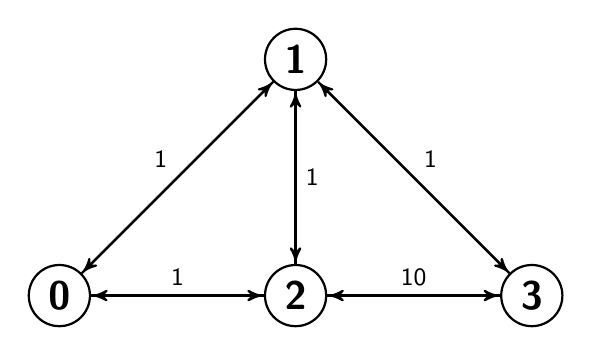
\begin{tikzpicture}[->,>=stealth',shorten >=1pt,auto,node distance=3cm,
                    thick,main node/.style={circle,draw,font=\sffamily\Large\bfseries}]

  \node[main node] (0) {0};
  \node[main node] (2) [right of=0] {2};
  \node[main node] (1) [above of=2] {1};
  \node[main node] (3) [right of=2] {3};

\path[every node/.style={font=\sffamily\small}]
    (0) edge node {1} (2)
        edge node {1} (1)
	(1) edge node {} (0)
        edge node {1} (2)
        edge node {1} (3)
    (2) edge node {} (0)
        edge node {} (1)
        edge node {10} (3)
    (3) edge node {} (2)
        edge node {} (1)
;
\end{tikzpicture}
\label{example:rip:1}
\caption{Example Of RIP solution 1}
\end{figure}
We will get the following initial path problem adjacency matrix by using the RIP protocol.
\[
\begin{bmatrix}
    \infty & 1 & 1 & \infty \\
    1 & \infty & 1 & 1 \\
    1 & 1 & \infty & 10 \\
    \infty & 1 & 10 & \infty \\
\end{bmatrix}
\]
After using the RIP protocol for matrix calculations (multiplication), we obtained such an adjacency matrix as the result:
\[
\begin{bmatrix}
    0 & 1 & 1 & 2 \\
    1 & 0 & 1 & 1 \\
    1 & 1 & 0 & 2 \\
    2 & 1 & 2 & 0 \\
\end{bmatrix}
\]
\begin{figure}[H]
\centering
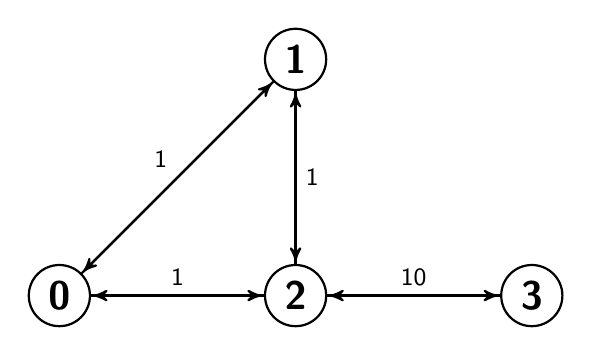
\begin{tikzpicture}[->,>=stealth',shorten >=1pt,auto,node distance=3cm,
                    thick,main node/.style={circle,draw,font=\sffamily\Large\bfseries}]

  \node[main node] (0) {0};
  \node[main node] (2) [right of=0] {2};
  \node[main node] (1) [above of=2] {1};
  \node[main node] (3) [right of=2] {3};

\path[every node/.style={font=\sffamily\small}]
    (0) edge node {1} (2)
        edge node {1} (1)
	(1) edge node {} (0)
        edge node {1} (2)
    (2) edge node {} (0)
        edge node {} (1)
        edge node {10} (3)
    (3) 
        edge node {} (2)
;
\end{tikzpicture}
\label{example:rip:2}
\caption{Example Of RIP solution 2}
\end{figure}
We will get the following initial path problem adjacency matrix by using the RIP protocol.
\[
\begin{bmatrix}
    \infty & 1 & 1 & \infty \\
    1 & \infty & 1 & \infty \\
    1 & 1 & \infty & 10 \\
    \infty & \infty & 10 & \infty \\
\end{bmatrix}
\]
After using the RIP protocol for matrix calculations (multiplication), we obtained such an adjacency matrix as the result:
\[
\begin{bmatrix}
    0 & 1 & 1 & 11 \\
    1 & 0 & 1 & 11 \\
    1 & 1 & 0 & 10 \\
    11 & 11 & 10 & 0 \\
\end{bmatrix}
\]

\section{Previous Problem in L11}
However, even so, RIP will also have a series of problems. For example, when a node does not have edges connected to it, the RIP matrix calculation (without pre-setting the maximum number of calculation steps) will continue infinitely. Even if the maximum number of calculation steps is set in advance, RIP still has some deficiencies in efficiency. 
This leads to the problem that not all real-world problems can be solved directly with the simple matrix semiring. 
For example, we may meet the following situation (node 3 is not connected to all other nodes).
\begin{figure}[H]
\centering
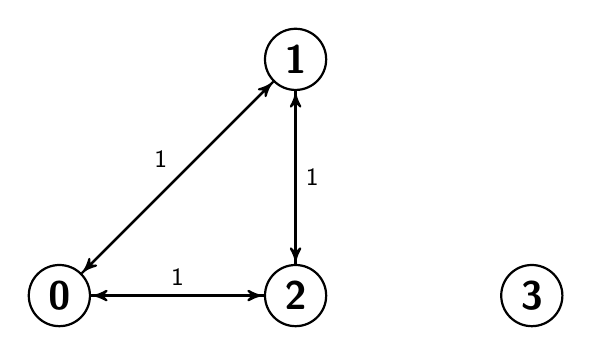
\begin{tikzpicture}[->,>=stealth',shorten >=1pt,auto,node distance=3cm,
                    thick,main node/.style={circle,draw,font=\sffamily\Large\bfseries}]

  \node[main node] (0) {0};
  \node[main node] (2) [right of=0] {2};
  \node[main node] (1) [above of=2] {1};
  \node[main node] (3) [right of=2] {3};

\path[every node/.style={font=\sffamily\small}]
    (0) edge node {1} (2)
        edge node {1} (1)
	(1) edge node {} (0)
        edge node {1} (2)
    (2) edge node {} (0)
        edge node {} (1)
;
\end{tikzpicture}
\label{example:rip:3}
\caption{Example Of RIP solution 3}
\end{figure}
We will get the following initial path problem matrix by using the RIP protocol.
\[
\begin{bmatrix}
    0 & 1 & 1 & \infty \\
    1 & 0 & 1 & \infty \\
    1 & 1 & 0 & \infty \\
    \infty & \infty & \infty & 0 \\
\end{bmatrix}
\]
After using the RIP protocol for n-step matrix calculations (multiplication), we obtained such a matrix:
\[
\begin{bmatrix}
    0 & 1 & 1 & n+1 \\
    1 & 0 & 1 & n+1 \\
    1 & 1 & 0 & n+1 \\
    \infty & \infty & \infty & 0 \\
\end{bmatrix}
\]
The result shows that if we do not limit the number of steps in the calculation, eventhough we may get the results of the path we need in the early step (eg path from $a$ to $b$), but a better solution for the entire matrix may be found after "many: steps (or the calculation will counting to infinity, which is shown in this example).
\subsection{Possible Solution}
Therefore, in the course L11, instead of using RIP and simple matrix semiring approach, we used another protocol called BGP. We start from the simple $(\mathbb{N},min,+)$ semiring that calculate the shortest distance, and we use lexicographic product (need reference to the Background/Definition) to construct a new semiring that contains the shortest-path metric and the set of its path.

Here we need to define some new operators/new rules for our semigroup.
Assume $(S,\bullet)$ is a semigroup. Let
\begin{equation}
  \label{eq:lift:def} 
  lift(S,\bullet)  \equiv (fin(2^S),\hat\bullet)
\end{equation}   
where
$X \hat\bullet Y = \{x\bullet y |x\in X,y\in Y\}$.

Then we can use our $lift$ to construct a bi-semigroup.
Assume $(S,\bullet)$ is a semigroup. Let
\begin{equation}
  \label{eq:unionlift:def} 
  union\_lift(S,\bullet)\equiv (\mathcal{P}(S),\cup,\hat\bullet)
\end{equation}  
where
$X \hat\bullet Y = \{x\bullet y |x\in X,y\in Y\}$, and $X,Y \in \mathcal{P}(S)$, which is the set of finite subsets of $S$.

Then for a given graph $G = (V,E)$, we define
\begin{equation}
  \label{eq:path:def} 
  path(E)\equiv union\_lift(E^*,.)
\end{equation}  
where . is the concatenation function of sequence.

Finally we get our "shortest paths with paths" semiring from a given graph $G = (V,E)$: 
\begin{equation}
  \label{eq:spwp:def} 
  spwp \equiv AddZero(\bar0,(\mathbb{N},min,+) \overrightarrow{\times} path(E))
\end{equation} 

\subsection{Introduce Reduction into Our Problem}
Here comes to the problem, when we are using $spwp$ for doing calculations, because there may have loops in our $path(E)$, we need a lot of extra computation (though it will eventually yield correct results) to prove the paths have loops are not the shortest path.
In order to eliminate these paths with loops, we introduced a new concept in the L11 course, the reduction.

If $(S,\oplus,\otimes)$ is a semiring and $r$ is a function from $S$ to $S$, then $r$ is a reduction if $\forall a,b \in S$, 
\[r(a) = r(r(a))\]
\[r(a\oplus b) = r(r(a)\oplus b) = r(a\oplus r(b))\] and 
\[r(a\otimes b) = r(r(a)\otimes b) = r(a\otimes r(b))\]

And, if $(S,\oplus,\otimes)$ is a semiring and $r$ is a reduction, then $red_r(S) = (S_r,\oplus_r,\otimes_r)$, where 
\[S_r = \{s\in S|r(s)= s\}\]
\[x\oplus_r y = r(x\oplus y)\]
\[x\otimes_r y = r(x\otimes y)\]

After that we went back to our path problem that for a given path $p$, we say $p$ is elementary if there is no node inside $p$ that is repeated. Then we can define our elementary path using the reduction 
\e{r:def:elementary}{r(X) = \{p\in X | p \mbox{ is elementary }\}}and 
\e{r:def:elementary_path}{epaths(E) = red_r(paths(E))}

Therefore, our path problem semiring became to 
\e{r:def:path_problem}{AddZero(\bar0,(\mathbb{N},min,+) \overrightarrow{\times} epath(E))}

However, we still encounter the problem that there exists elements in our problem set that has a path distance value but does not have edges in its path. So we need to define the second reduction, which turns all elements that don't satisfy the condition into a single element (the $zero$ we added into our semiring).
\e{r:def:reduction_annihilator}{
\begin{array}{rcl} 
r_2 (inr(\infty)) & = & inr(\infty) \\
r_2 (inl(s,\{\})) & = & inr(\infty) \\
r_2 (inl(s,W))    & = & inl(s,W) \\
\end{array}}
Therefore, our path problem semiring becomes to 
\e{r:def:reduced_path_problem}{red_{r_2}(AddZero(\bar0,(\mathbb{N},min,+) \overrightarrow{\times} epath(E)))}

It is worth mentioning that we did not discuss the properties of reduction in detail in the L11 course. We also did not know whether the original semiring still satisfies the semiring property after the reduction. At the same time, whether some properties of the original operators (such as commutative rules) remains or not after reduction is also a mystery to us.

These are the topics that we need to focus on in our discussion.
It is worth mentioning that the first reduction (reduce all pathes that are not elementary) that we defined above does not follow the property of the reduction on the $min$ operation (doesn't have left/right invariant property). Imagine we have path $A = \{a,b,c,d\}$ that is longer but does not have loop and $B = \{a,b,b\}$ that is shorter but does have loop. Then $r(A\oplus B) = r(B) = \infty$ because $B$ is shorter but has loop, but $r(A\oplus r(B)) = r(A \oplus \infty) = r(A) = A$ because $B$ has loops but $A$ doesn't.

Therefore, we not only discuss the properties of reduction, but also try to find another way to represent reduction to solve our path problem.



%\chapter{Related Work} 
%
%This chapter covers relevant (and typically, recent) research 
%which you build upon (or improve upon). There are two complementary 
%goals for this chapter: 
%\begin{enumerate} 
%  \item to show that you know and understand the state of the art; and 
%  \item to put your work in context
%\end{enumerate} 
%
%Ideally you can tackle both together by providing a critique of
%related work, and describing what is insufficient (and how you do
%better!)
%
%The related work chapter should usually come either near the front or
%near the back of the dissertation. The advantage of the former is that
%you get to build the argument for why your work is important before
%presenting your solution(s) in later chapters; the advantage of the
%latter is that don't have to forward reference to your solution too
%much. The correct choice will depend on what you're writing up, and
%your own personal preference.

\chapter{Mathematical Reasoning and Coq Implementation} 

%This chapter may be called something else\ldots but in general 
%the idea is that you have one (or a few) ``meat'' chapters which
%describe the work you did in technical detail. 

\section{Classical Reduction, Example and Reasoning}
\subsection{Origin of the Concept of Reduction.}
In order to better understand reduction and further analyze it in detail, we trace the source to find out if there is any other definition and study of reduction before us. 
In fact, the earliest definition we could find about reduction came from Ahnont Wongseelashote in 1977\cite{WONGSEELASHOTE197955}. Wongseelashote also encountered the problem similar to ours when studying the path problem in the paper. In fact, our definition of reduction is very similar to Wongseelashote's definition of reduction (the real reason is that L11 refers to the Wongseelashote definition when the definition of reduction was given). However, unfortunately, Wongseelashoth only put forward the concept of reduction in the paper without detailed reasoning and structure proof.

Next we found that Alexander James Telford Gurney also mentioned the concept of reduction in his Ph.D thesis\cite{gurney_construction_2010}. Gurney's discussion of reduction is also based on the definition by Wongseelashote, and it also does not focus on reduction for detailed structure proof.

\subsection{Classical Reduction Definition}
Therefore, here we refer to the definition of reduction in L11 (also the definition of Wongseelashote in paper) as the classical reduction, and we give the name of the way in which Wongseelashote represented reduction in paper as the traditional representation of reduction.
\begin{figure}[H]
\centering
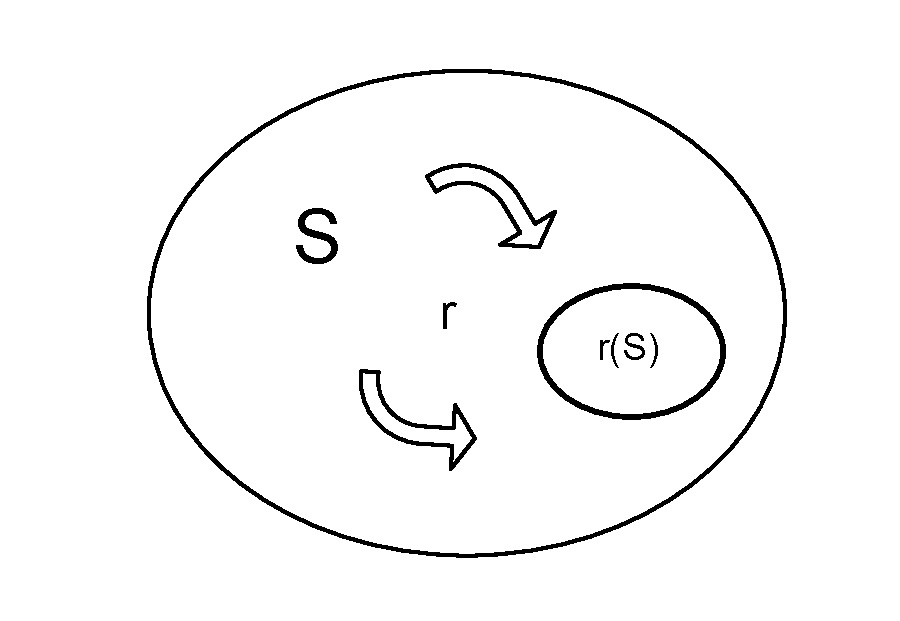
\includegraphics[width=0.8\textwidth]{reduction.pdf}
\label{reduction}
\caption{Illustration of Reduction}
\end{figure}
For a problem set $S$, the reduced problem set under reduction $r: S \rightarrow S$ is represented as 
\e{r:def:traditional}{r(S) \equiv \{s \in S | r(s) =_S s\}}
Then for the problem set $S$ that represented as a semirgroup $(S,=_S,\oplus)$, the reduced problem set will be represented as $({r(S) \equiv \{s \in S | r(s) =_S s\}},=_S,\oplus_r)$ where 
\e{r:def:binary_operator}{\forall a, b \in \{r(S) \equiv \{s \in S | r(s) =_S s\}, a \oplus_r b \equiv r(a \oplus b)}
It is worth mentioning that although we use reduction to reduce the problem set from $S$ to $\{r(S) \equiv \{s \in S | r(s) =_S s\}$, our equality $=_S$ is still the original equality $=_S$, .
This can be seen from the figure (\ref{reduction}), although we currently only focus on a subset of the original problem set $S$, the equality established on the problem set is still established on this subset.
Here as the reduction $r$ need to have the following properties.

Congruence: \e{r:def:congruence}{\forall a,b \in S, a =_S b \rightarrow r(a) =_S r(b)}
Idempotent: \e{r:def:idempotent}{r(a) = r(r(a))} 
Left Invariant: \e{r:def:left_invariant}{r(a\oplus b) = r(r(a)\oplus b) = r(a\oplus r(b))}
Right Invariant: \e{r:def:right_invariant}{r(a\otimes b) = r(r(a)\otimes b) = r(a\otimes r(b))}

\subsection{Example on L11 Lecture}
To help us understand reduction and study its properties, we found another example of reduction in the course of L11.

The reduction is call $min_{\leq}$ (Martelli’s semiring)\cite{martelli_gaussian_1976} which means removing all the superset.
For a given graph $G = (V,E)$, A cut set $C \in E$ for nodes $i$ and $j$ is a set of edges such there is no path from $i$ to $j$ in the graph $(V, E - C)$. $C$ is minimal if no proper subset of $C$ is a cut set. And Martelli’s semiring is such that $A^{(*)}(i, j)$ is the set of all minimal cut sets for $i$ and $j$. 
So Martelli’s semiring is represented as \[(S,\oplus,\otimes,\bar0,\bar1)\] where \[S = min_\leq(2^{2^E})\] \[X\oplus Y = min_\leq(\{U \cup V | U \in X, V \in Y\})\] \[X\otimes Y = min_\leq(X \cup Y)\] \[\bar0 = \{\{\}\}\] \[\bar1 = \{\}\]
Here we can easily prove that $min_\leq$ satisfies our previous definition of reduction. So $min_\leq$ is a classical reduction.
\subsection{Reasoning on Classical Reduction}
Next we need to make a detailed reasoning the properties of the reduction.
Because we are talking about classical reduction, we assume that our reduction $r$ has properties of congruence (\ref{r:def:congruence}), idempotent (\ref{r:def:idempotent}), left invariant (\ref{r:def:left_invariant}) and right invariant (\ref{r:def:right_invariant}).

First we discuss the properties of equality on reduction set. We assume the equality $=_S$ has the properties of reflexive (\ref{def:eq:reflexive}), symmetric (\ref{def:eq:symmetric}), transitive (\ref{def:eq:transitive}) and congruence (\ref{def:eq:congruence}) on the original problem set $S$.
Then in the definition of our reduction representation we mentioned "although we use reduction to reduce the problem set from $S$ to $\{r(S) \equiv \{s \in S | r(s) =_S s\} $, we equality $=_S$ is still the original equality $=_S$”, so on reduced problem set $\{r(S) \equiv \{s \in S | r(s) =_S s\}$ ,the equality $=_S$ still has the property of reflexive, symmetric, transitive and congruence.

Next we need to discuss the properties of the binary operator under reduced problem set. 
Recalling to our definition, for a binary operator $\oplus : S \times S \rightarrow S$, the reduced binary operator under reduction $r$ is defined as \[\forall a, b \in \{r(S) \equiv \{s \in S | r(s) =_S s\}, a \oplus_r b \equiv r(a \oplus b)\]
So we first assume that the original binary operator $\oplus$ has certain properties on $S$, and then reasoning that these properties are remained after reduction ($\oplus_r$ still has the same property under $\{r(S) \equiv \{s \in S | r(s) =_S s\}$)

Commutative: we initially assume that $\oplus$ is commutative under $S$, which is $\forall a,b \in S, a \oplus b =_S b \oplus a$. Then we want to proof that $\forall a,b \in \{s \in S | r(s) =_S s\}, a \oplus_r b =_S b \oplus_r a$.
\e{r:proof:commutative}{
\begin{array}{rcll} 
a \oplus_r b & =_S & r(a \oplus b) &\mbox{by the definition of $\oplus_r$} \\
			 & =_S & r(b \oplus a) &\mbox{by commutative of $\oplus$ and congruence of $r$}\\
             & =_S & b \oplus_r a &\mbox{by the definition of $\oplus_r$} \\
\end{array}}
So we can conclude that commutative of $\oplus$ plus congruence of $r$ implies commutative of $\oplus_r$.

Congruence: we initially assume that $\oplus$ is congruence under $S$, which is $\forall a,b,c,d \in S, a =_S b \wedge c =_S d \rightarrow a \oplus c =_S b \oplus d$. Then we want to proof that $\forall a,b,c,d \in \{s \in S | r(s) =_S s\}, a =_S b \wedge c =_S d \rightarrow a \oplus_r c =_S b \oplus_r d$.
\e{r:proof:congruence}{
\begin{array}{rcll} 
a \oplus_r c & =_S & r(a \oplus c) &\mbox{by the definition of $\oplus_r$} \\
			 & =_S & r(b \oplus c) &\mbox{by congruence of $\oplus$ and congruence of $r$}\\
			 & =_S & r(b \oplus d) &\mbox{by congruence of $\oplus$ and congruence of $r$}\\
             & =_S & b \oplus_r d &\mbox{by the definition of $\oplus_r$} \\
\end{array}}
So we can conclude that congruence of $\oplus$ plus congruence of $r$ implies congruence of $\oplus_r$.

Selective: we initially assume that $\oplus$ is selective under $S$, which is $\forall a,b \in S, a \oplus b =_S a \bigvee a \oplus b =_S b$. Then we want to proof that $\forall a,b \in \{s \in S | r(s) =_S s\}, a \oplus_r b =_S a \bigvee a \oplus_r b =_S b$. By using the selective property, we can split the cases of $a\oplus b$.

case 1: $a \oplus b =_S a$
\[
\begin{array}{rcll} 
a \oplus_r b & =_S & r(a \oplus b) &\mbox{by the definition of $\oplus_r$} \\
			 & =_S & r(a) &\mbox{congruence of $r$}\\
			 & =_S & a &\mbox{because $r(a) = a$}\\
\end{array}
\]
case 2: $a \oplus b =_S b$
\[
\begin{array}{rcll} 
a \oplus_r b & =_S & r(a \oplus b) &\mbox{by the definition of $\oplus_r$} \\
			 & =_S & r(b) &\mbox{congruence of $r$}\\
			 & =_S & b &\mbox{because $r(b) = b$}\\
\end{array}
\]
So we can conclude that selective of $\oplus$ plus congruence of $r$ implies selective of $\oplus_r$.

Associative: we initially assume that $\oplus$ is associative under $S$, which is $\forall a,b,c \in S, a \oplus (b \oplus c) =_S (a \oplus b) \oplus c$. Then we want to proof that $\forall a,b,c \in \{s \in S | r(s) =_S s\}, a \oplus_r (b \oplus_r c) =_S (a \oplus_r b) \oplus_r c$. 
\e{r:proof:associative}{
\begin{array}{rcll} 
a \oplus_r (b \oplus_r c) & =_S & r(a \oplus r(b \oplus c)) &\mbox{by the definition of $\oplus_r$} \\
			 & =_S & r(a \oplus (b \oplus c)) &\mbox{by right invariant property of $r$ on $\oplus$}\\
			 & =_S & r((a \oplus b) \oplus c) &\mbox{by associative of $\oplus$ and congruence of $r$}\\
			 & =_S & r(r(a \oplus b) \oplus c) &\mbox{by left invariant property of $r$ on $\oplus$}\\
             & =_S & (a \oplus_r b) \oplus_r c  &\mbox{by the definition of $\oplus_r$} \\
\end{array}}
So we can conclude that associative of $\oplus$ plus congruence, left and right invariant of $r$ on $\oplus$ implies associative of $\oplus_r$.
Here we find that associative is not the same as the other three properties under binary operators. The proof that a binary operator satisfies the associative under reduction uses the left/right invariant properties of reduction. And in the later section we will focus on the properties of the associative and do reasoning on it. 

Left Distributive: by adding another binary operator $\otimes : S \times S \rightarrow S$, the reduced binary operator $\otimes_r$ as $\forall a,b \in \{s \in S | r(s) =_S s\}, a \otimes_r b \equiv r(a \otimes b)$, we initially assume that $\oplus$ and $\otimes$ are left distributive under $S$, which is $\forall a,b,c \in S, a \otimes (b \oplus c) =_S (a \otimes b) \oplus (a \otimes c)$. Then we want to proof that $\forall a,b,c \in \{s \in S | r(s) =_S s\}, a \otimes_r (b \oplus_r c) =_S (a \otimes_r b) \oplus_r (a \otimes_r c)$. 
\e{r:proof:left_distributive}{
\begin{array}{rcll} 
a \otimes_r (b \oplus_r c) & =_S & r(a \otimes r(b \oplus c)) &\mbox{by the definition of $\oplus_r$ and $\otimes_r$} \\
			 & =_S & r(a \otimes (b \oplus c)) &\mbox{by right invariant property of $r$ on $\otimes$}\\
			 & =_S & r((a \otimes b) \oplus (a \otimes c)) &\mbox{by left distributive of $\oplus$ and $\otimes$}\\
			 & =_S & r(r(a \otimes b) \oplus r(a \otimes c)) &\mbox{by left and right invariant of $r$ on $\oplus$}\\			 
			 & =_S & r((a \otimes_r b) \oplus (a \otimes_r c)) &\mbox{by the definition of $\otimes_r$}\\
             & =_S & (a \otimes_r b) \oplus_r (a \otimes_r c)  &\mbox{by the definition of $\oplus_r$} \\
\end{array}}
So we can conclude that left distributive of $\oplus$ and $\otimes$ plus congruence, left and right invariant of $r$ on $\oplus$, right invariant of $r$ on $\otimes$ implies left distributive of $\oplus_r$ and $\otimes_r$.

Similarly we can conclude that right distributive of $\oplus$ and $\otimes$ plus congruence, left and right invariant of $r$ on $\oplus$, left invariant of $r$ on $\otimes$ implies right distributive of $\oplus_r$ and $\otimes_r$.

Thus, we get the conclusion that distributive of $\oplus$ and $\otimes$ plus congruence, left and right invariant of $r$ on $\oplus$ and $\otimes$ implies distributive of $\oplus_r$ and $\otimes_r$.
It is also worth mentioning that the property of the distributive is also one of the major features we will discuss in the later section.

\section{New Reduction Representation}
The previous section have mentioned that our definition of classical reduction traditional representation is implementation unfriendly.

This is because inside traditional reduction representation our actual problem set is $r(S) = \{s\in S|r(s)=_S s\}$ which is a type with record. Record is difficult to be accurately represented in most situations. 

Imagine we have two different reductions $r_1$ and $r_2$ for $S$, then the problem set after applying reduction $r_1$ and $r_2$ will be $r_2(r_1(S)) = \{y\in \{x \in S | r_1(x) =_S x\}|r_2(y)=_S y\}$. 

The nest record of reduction in our problem domain makes all the reasoning and calculation step into trouble. 
At the same time, since our real problem set has changed from the original $S$ to the current $r(S) = \{s\in S|r(s)=_S s\}$ (suppose we only have one reduction $r$), the domain of our binary operator has changed. If we originally have a binary operator $\oplus : S\times S \rightarrow S$, then the binary operator after reduction will become the binary operator \[\oplus_r : \{s\in S|r(s)=_S s\} \times \{s\in S|r(s)=_S s\} \rightarrow \{s\in S|r(s)= s\}\] And if we apply two/more reductions simultaneously, the entangling of reductions with problem set and operator makes it almost impossible for us to define the combinator that exists on reduction and solve the problem at all.

Our goal is to redefine the equality and binary operators without changing the problem set $S$. 
Then the reduced problem set based on $(S,=_S,\oplus)$ by reduction $r$ will become $(S,=^r_S,\oplus^r)$, which is still a problem set on $S$, but not $(\{x \in S | r(x) =_S x\}, =,\oplus_r)$. 
Then we will prove the isomorphism between these two representations.

\subsection{Generalized Representation of Equality and Binary Operator}
Let us look back and forth at the figure (\ref{reduction}). In the figure, our reduction will reduce the problem set $S$ to a subset of $S$. In our traditional representation, because reduction has already brought problem set from $S$ to $\{x \in S | r(x) =_S x\}$, which means when we are comparing two elements from the problem set, those two elements are already inside $\{x \in S | r(x) =_S x\}$, we can directly use the original equality $=_S$ as well.

However if we want to keep our problem set still as $S$, when we are doing equality comparison, we must guarantee that the elements we compared are already inside the reduced problem set. Thus we defined the new equality as
\e{gr:def:eq}{\forall a,b \in S, a =^r_S b \equiv r(a) =_S r(b)}

The same reason for our binary operator $\oplus$, when we defined $\oplus_r$ earlier, because the arguments we need have been reduced to $\{x \in S | r(x) =_S x \}$, we only need to consider that the result of operation must also be in $\{x \in S | r(x) =_S x\}$, so we give the definition above (\ref{r:def:binary_operator}).

Similarly to the equality, if we want to keep our problem set still as $S$, when we are doing binary operation, we not only need to consider that the result of the operation is in the reduced problem set, we also need to ensure that the two arguments of the binary operator are in the reduced problem set. Therefore we define our binary operator under reduction:
\e{gr:def:binary_operator}{\forall a,b \in S, a \oplus^r b \equiv r(r(a) \oplus r(b))}

\subsection{Isomorphism between Transitional and Generalized Representation}
Next we need to prove that our new generalized representation is isomorphic to the previous traditional representation.

\subsubsection{Isomorphic On Equality Properties}
First we discuss the properties on equality between the traditional representation and the generalized representation.

Congruence: we need to proof that $=_S$ is congruence on $\{x \in S | r(x) =_S x\}$ is isomorphic to $=^r_S$ is congruence on $S$, which means 
\[\forall a,b,c,d \in \{x \in S | r(x) =_S x \}, a =_S b \wedge c =_S d \rightarrow a =_S c = b =_S d \]
\[\longleftrightarrow \]
\[\forall a,b,c,d \in S, a =^r_S b \wedge c =^r_S d \rightarrow a =^r_S c = b =^r_S d
\]

Reflexive: we need to proof that $=_S$ is reflexive on $\{x \in S | r(x) =_S x \}$ is isomorphic to $=^r_S$ is reflexive on $S$, which means 
\[\forall a \in \{x \in S | r(x) =_S x \}, a =_S a \]
\[\longleftrightarrow \]
\[\forall a \in S, a =^r_S a
\]

Symmetric: we need to proof that $=_S$ is symmetric on $\{x \in S | r(x) =_S x\}$ is isomorphic to $=^r_S$ is symmetric on $S$, which means 
\[\forall a,b \in \{x \in S | r(x) =_S x \}, a =_S b \rightarrow b =_S a \]
\[\longleftrightarrow \]
\[\forall a,b \in S, a =^r_S b \rightarrow b =^r_S a
\]

Transitive: we need to proof that $=_S$ is transitive on $\{x \in S | r(x) =_S x \}$ is isomorphic to $=^r_S$ is transitive on $S$, which means 
\[\forall a,b,c \in \{x \in S | r(x) =_S x \}, a =_S b \wedge b =_S c \rightarrow a =_S c \]
\[\longleftrightarrow \]
\[\forall a,b,c \in S, a =^r_S b \wedge b =^r_S c \rightarrow a =^r_S c
\]

These proof are really trivial and only need the property of idempotent of $r$, which is $\forall a \in S, r(a) = r(r(a))$.

\subsubsection{Isomorphic On Binary Operator Properties}
Next we discuss the properties on binary operator $\oplus$ (and $\otimes$ when we are talking about distributive) between the traditional representation and the generalized representation.

Commutative: we need to proof that $\oplus_r$ is commutative on $\{x \in S | r(x) =_S x\}$ is isomorphic to $\oplus^r$ is commutative on $S$, which means 
\[\forall a,b \in \{x \in S | r(x) =_S x \}, a \oplus_r b =_S b \oplus_r a \]
\[\longleftrightarrow \]
\[\forall a,b \in S, a \oplus^r b =^r_S b \oplus^r a
\]

Selective:  we need to proof that $\oplus_r$ is selective on $\{x \in S | r(x) =_S x\}$ is isomorphic to $\oplus^r$ is selective on $S$, which means 
\[\forall a,b \in \{x \in S | r(x) =_S x\}, a \oplus_r b =_S a \bigvee a \oplus_r b =_S b \]
\[\longleftrightarrow \]
\[\forall a,b \in S, a \oplus^r b =^r_S a \bigvee a \oplus^r b =^r_S b
\]

Congruence: we need to proof that $\oplus_r$ is congruence on $\{x \in S | r(x) =_S x\}$ is isomorphic to $\oplus^r$ is congruence on $S$, which means 
\[\forall a,b,c,d \in \{x \in S | r(x) =_S x \}, a =_S b \wedge c =_S d \rightarrow a \oplus_r c =_S b \oplus_r d \]
\[\longleftrightarrow \]
\[\forall a,b,c,d \in S, a =^r_S b \wedge c =^r_S d \rightarrow a \oplus^r c =^r_S b \oplus^r d
\]

Associative: we need to proof that $\oplus_r$ is associative on $\{x \in S | r(x) =_S x\}$ is isomorphic to $\oplus^r$ is associative on $S$, which means 
\[\forall a,b,c \in \{x \in S | r(x) =_S x \}, a \oplus_r (b \oplus_r c) =_S (a \oplus_r b) \oplus_r c \]
\[\longleftrightarrow \]
\[\forall a,b,c \in S, a \oplus^r (b \oplus^r c) =^r_S (a \oplus^r b) \oplus^r c
\]

Left Distributive: we need to proof that $\oplus_r$ and $\otimes_r$ are left distributive on $\{x \in S | r(x) =_S x\}$ is isomorphic to $\oplus^r$ and $\oplus^r$ are left distributive on $S$, which means 
\[\forall a,b,c \in \{x \in S | r(x) =_S x \}, a \otimes_r (b \oplus_r c) =_S (a \otimes_r b) \oplus_r (a \otimes_r c) \]
\[\longleftrightarrow \]
\[\forall a,b,c \in S, a \otimes^r (b \oplus^r c) =^r_S (a \otimes^r b) \oplus^r (a \otimes^r c)
\]

Right Distributive: we need to proof that $\oplus_r$ and $\otimes_r$ are right distributive on $\{x \in S | r(x) =_S x\}$ is isomorphic to $\oplus^r$ and $\oplus^r$ are right distributive on $S$, which means 
\[\forall a,b,c \in \{x \in S | r(x) =_S x \}, (a \oplus_r b) \otimes_r c =_S (a \otimes_r c) \oplus_r (b \otimes_r c) \]
\[\longleftrightarrow \]
\[\forall a,b,c \in S, (a \oplus^r b) \otimes^r c =^r_S (a \otimes^r c) \oplus^r (b \otimes^r c)
\]

These proof will be shown in Coq file and we only need the property of congruence and idempotent of $r$, which is $\forall a \in S, r(a) = r(r(a))$ and $\forall a,b \in S, a =_S b \rightarrow r(a) =_S r(b)$.

This proves that our generalized representation of reduction is isomorphic to the traditional representation of reduction, which means all the properties we have proved in the classical reduction section could be used directly into our generalized representation.

\section{Generalized Reduction}
In our previously defined classical reduction (either in traditional representation or generalized representation), reduction must satisfy four properties that it is congruence, idempotent, left and right invariant. However, the reduction we encounter in reality does not all have the above four properties, especially the left/right invariant properties. In particular, the elementary reduction in the elementary path problem that we mentioned earlier, which will also be used in the later section to construct our final path problem, does not satisfy the properties of the left/right invariant on the $min$ operator. 

Assuming $P_1,P_2 \in Path, P_1 \leq P_2, loop(P_1) = true \wedge loop(P_2) = false$. 
Then $r(min(P_1,P_2)) = r(P_1) = \infty$.
However $r(min(r(P_1),P_2)) = r(min(\infty,P_2)) r(P_2) = P_2$. 

Therefore, in order to define our elementary path reduction and also to better represent other reductions, we generalize the definition reduction as: $r$ is a reduction on $S$ if $r$ has the properties of congruence and idempotent, and get rid of the constraint of left/right invariant properties, and we name this kind of reduction as generalized reduction.

Do not confuse generalized representation of reduction with generalized reduction here. 
Generalized representation of reduction is a new representation of reduction, compared to and isomorphic to the traditional representation of reduction, that is implementation friendly. A reduction that represented by generalized representation could be classical reduction (that has left/right invariant properties) or generalized reduction (left/right invariant properties can be gotten rid of).
Generalized reduction we defined here is a kind of reduction that is only asked for idempotent and congruence properties without forced to be left/right invariant. Generalized reduction could be represented by using traditional representation or generalized representation.

Because the generalized representation is implementation friendly, and we have proved the isomorphism between the generalized representation and traditional representation, we will use generalized representation to represent reduction in the following paragraph.

\subsection{Properties of Generalized Reduction, Pseudo Associative and Pseudo Distributive}
We have reasoned about the relationship between reduction and equality/binary operators in the previous section of classical reduction. 
Since in the last section we have already reached a grossized representation is isomorphic to the traditional representation, and the generalized reduction is just the classical reduction without left/right invariant properties, by assuming that the reduction $r$ is congruence and idempotent, we can have the following conclusion:

If $=_S$ is congruence/reflexive/symmetric/transitive on the problem set $S$, then $=^r_S$ is congruence/reflexive/symmetric/transitive on the problem set $S$.

If $\oplus$ has the properties of commutative/selective/congruence on the problem set $S$, then $\oplus^r$ has the properties of commutative/selective/congruence on the problem set $S$.

There is another property that we may be interested in, if $i$/$a$ is the identity/annihilator for $\oplus$ on $S$, and the reduction $r$ has the properties of preserve id/ann (\ref{def:uop:preserve_id},\ref{def:uop:preserve_ann}), then $i$/$a$ is the identity/annihilator for $\oplus^r$ on $S$.

The more troublesome is the properties of associative and distributive. Since the proof used the property of left/right invariant, and we don't have those properties inside generalized reduction by default, we cannot directly get the these two properties. So we conclude that generalized reduction with left/right properties will allow the operator(s) remaining associative and distributive properties.

However, the elementary path reduction we want to define afterwards is only a generalized reduction and does not have left/right invariant properties on the $min$ operator. We still want to discuss the properties and relationship between the reduction and the operator and discuss whether $min$ has associative property under reduction, and discuss whether the entire semiring has distributive properties.

Therefore, we found two sufficient condition, separately for associative properties and distributive properties respectively that we can prove the properties if we can prove the sufficient condition is holding.

Pseudo Associative:
\e{gr:def:pseudo_associative}{\forall a,b,c \in S, r(r(r(a)\oplus r(b)) \oplus r(c)) = r(r(a) \oplus r(r(b)\oplus r(c)))}
Pseudo Left Distributive: 
\e{gr:def:pseudo_left_distributive}{\forall a,b,c \in S, r(r(a) \otimes r(r(b)\oplus r(c))) = r(r(r(a) \otimes r(b)) \oplus r(r(a) \otimes r(c)))}
Pseudo Right Distributive: 
\e{gr:def:pseudo_right_distributive}{\forall a,b,c \in S, r(r(r(a) \oplus r(b)) \otimes r(c)) = r(r(r(a) \otimes r(c)) \oplus r(r(b) \otimes r(c)))}
It is easy to prove $\oplus^r$ is associative on $S$, and $\oplus^r$ and $\otimes^r$ are distributive on $S$ by using pseudo associative and pseudo distributive properties.

Associative: by definition of $=^r_S$, $\oplus^r$
\[
\forall a,b,c \in S, a \oplus^r (b \oplus^r c) =^r_S (a \oplus^r b) \oplus^r c
\]
\[\longleftrightarrow \]
\[
	r(r(r(a) \oplus r(r(r(b) \oplus r(c))))) =_S r(r(r(r(r(a) \oplus r(b))) \oplus r(c)))
\]
$r(r(r(a) \oplus r(r(r(b) \oplus r(c)))))$
\e{gr:proof:associative}{
\begin{array}{rcll}
	 & =_S & r(r(a) \oplus r(r(r(b) \oplus r(c)))) & \mbox {by idempotent property of $r$} \\
	& =_S & r(r(a) \oplus r(r(b) \oplus r(c))) & \mbox {by idempotent property of $r$ and congruence of $\oplus$}\\
	 & =_S & r(r(r(a)\oplus r(b)) \oplus r(c)) & \mbox {by pseudo associative}\\
	 & =_S & r(r(r(r(a)\oplus r(b))) \oplus r(c)) & \mbox {by idempotent property of $r$ and congruence of $\oplus$}\\
	 & =_S & r(r(r(r(r(a)\oplus r(b))) \oplus r(c))) & \mbox {by idempotent property of $r$}\\
\end{array}
}

Left Distributive: by definition of $=^r_S$, $\oplus^r$ and $\otimes^r$
\[
\forall a,b,c \in S, a \otimes^r (b \oplus^r c) =^r_S (a \otimes^r b) \oplus^r (a \otimes^r c)
\]
\[\longleftrightarrow \]
\[
	r(r(r(a)) \otimes r(r(r(b) \oplus r(c))))) =_S r(r(r(r(r(a) \otimes r(b))) \oplus r(r(r(a) \otimes r(c)))))
\]
$r(r(r(a)) \otimes r(r(r(b) \oplus r(c)))))$
\e{gr:proof:left_distributive}{
\begin{array}{rcll}
	 & =_S & r(r(a) \otimes r(r(b) \oplus r(c)))) & \mbox {by idempotent property of $r$ and congruence of $\otimes$} \\
	 & =_S & r(r(r(a) \otimes r(b)) \oplus r(r(a) \otimes r(c))) & \mbox {by pseudo left distributive} \\
	 & =_S & r(r(r(r(a) \otimes r(b))) \oplus r(r(r(a) \otimes r(c)))) & \mbox {by idempotent property of $r$ and congruence of $\oplus$} \\
	 & =_S & r(r(r(r(r(a) \otimes r(b))) \oplus r(r(r(a) \otimes r(c))))) & \mbox {by idempotent property of $r$} \\
\end{array}
}

Similar proof for right distributivity. 

So we can conclude that for generalized reduction, although it may not have the property of left/right invariant, if we can directly prove the properties of pseudo associative/pseudo distributive, then we can also prove that binary operator(s) remains associative/distributive under reduction.

\section{Predicate Reduction}
In order to better implement the construction of the path problem we mentioned earlier, we are going to define a type of reduction and perform detailed reasoning on its properties in this section. 
If we deeply consider our reduction, whether it is to eliminate the path with a loop, or to turn an unqualified element tuple into a specific element -- additive identity/multiplicative annihilator, we can easily find the situation that our reduction is depending on a predicate and reducing the elements that satisfy/not satisfy the condition. Therefore, we call this kind of reduction as predicate reduction.

We define a new type of reduction, predicate reduction based on generalized reduction. 
Predicate reduction is a kind of generalized reduction, but it is not as much generalized as the generalized reduction. Generalized reduction could define almost all kinds of reductions, but predicate reduction couldn't, and it is the reason why it is not as much generalized as the previous one. For example, when we are talking about the min set $min_\leq = \{ x \in X | \forall y \in X, y \not\leq x \}$, which is introduced as Martelli’s semiring in our previous section, we can't define $min_\leq$ using predicate reduce. The reason is, when we are defining a predicate, the predicate only know the information on its current element, but not the whole problem set. Predicate reduction is still a kind of generalized reduction but not classical reduction because it is not forcing the reduction to have left/right invariant properties. Have or not those properties depends on the predicate inside reduction. For example, we will use predicate reduction to define three different reductions in the later section, two of them (min plus with ceiling and reduction annihilator) has the properties of left/right invariant on both operator, but one of them (elementary path) doesn't on its $min$ operator.

Here comes to our definition. Initially for our problem set $S$, we define a predicate $P$, which is a function from $S$ to $bool$ and we need to provide a specific element $c$ (the predicate reduction will reduce all the element that satisfied the predicate to $c \in S$). Then we can define the predicate reduction as 
\e{pr:def:def}{\forall a \in S,  r_p(a)=\left\{
\begin{aligned}
c &  & P(a) = true \\
a &  & otherwise 
\end{aligned}
\right.}

As we mentioned previously, predicate reduction is defined based on the generalized reduction, which means it has all the properties that generalized reduction has. Hence, we are not interested on the properties of equality, congruence, commutative and selective, has identity and has annihilator properties of binary operator any more. We mainly talk about the associative and distributive in the reasoning section (although we may use the properties of has identity and has annihilator during the process of proof).

\subsection{Properties of Predicate}
In predicate reduction, we hope to explore the properties of predicate reduction that are different from generalized reduction.
But as the predicate reduction is a kind of generalized reduction, it must have the properties of the idempotent and congruence property, which are $\forall a \in S, r(a) = r(r(a))$ and $\forall a,b\in S, a = b \rightarrow r(a) = r(b)$. So we need to do reasoning on these two properties. For the property of the idempotent, we need to discuss the input element, split the case that the element satisfies the predicate or not. If the element doesn't satisfy the predicate, then $r(a) = a = r(r(a))$. If the element does satisfy the predicate, then $r(a) = c$ and $r(r(a)) = r(c)$, hence we need to prove/provide the property that $c$ must satisfy the predicate \e{pr:proof:p_true}{P(c) = true}
For the property of the congruence, we can conclude from 
\[\forall a,b \in S, r_p(a)=\left\{
\begin{aligned}
c &  & P(a) = true \\
a &  & otherwise 
\end{aligned}
\right. = 
r_p(b)=\left\{
\begin{aligned}
c &  & P(b) = true \\
b &  & otherwise 
\end{aligned}
\right.\] that we need such a property \e{pr:proof:p_cong}{\forall a,b \in S, a = b \rightarrow P(a) = P(b)} which is the congruence of the predicate $P$.

Next we need to reduce the binary operator according to the generalize representation we defined earlier using the predicate reduction. For our problem set $S$ and a given binary operator $\oplus$, we defined reduced binary operator as 
\e{pr:def:binary_operator}{\forall a,b \in S, a \oplus_r b = r_p (r_p(a) \oplus r_p(b))}

Therefore, here we mainly discuss the properties of predicates and their relationship with binary operators, and then try to prove associative/distributive by using pseudo associative/distributive without forcing the left/right invariant on the reduction. In this process we discovered three very interesting properties about predicates. 

Before describing these three properties, we first introduce an implicit definition. If our operator is selective, then we actually implicitly define a partial order on the problem set.
\[\forall a,b \in S, a \oplus b =_S a \leftrightarrow a \leq b\]

Next we begin to formally introduce our three properties for the predicate.

Decomposition: \e{pr:def:decomposition}{\forall a,b \in S, P(a \oplus b)= true \rightarrow P(a) = true \bigvee P (b) = true}
Composition: \e{pr:def:composition}{\forall a,b \in S, P(a) = true \bigvee P (b) = true \rightarrow P(a \oplus b)= true}
Preserve Order: \e{pr:def:preserve_order}{\forall a,b \in S, a \leq b \wedge P(a) = true \rightarrow P(b) = true}
From the property of decomposition we can infer that \e{pr:proof:decomposition_contra}{\forall a,b \in S, P(a) = false \bigwedge P (b) = false \rightarrow P(a \oplus b)= false} which means the binary operator will not create elements that satisfy the predicate condition from the elements that don't satisfy the condition.

From the property of decomposition we can infer that \e{pr:proof:composition_contra}{\forall a,b \in S, P(a \oplus b)= false \rightarrow P(a) = false \bigwedge P (b) = false} which means the result of the binary operation will decide the predicate condition of its arguments.

Generally speaking, because our additive component of the semiring is mostly selective, then most of our additive components have decomposition properties, and we are mostly concerning about whether our additive component preserving the order or not. At the same time, because our multiplicative component always plays the role of an accumulator, which makes the composition property important for multiplicative components.

Let us discuss the above two properties at the level of reduction. If a predicate is decomposed/composition on an operator, it means that the reduction formed by this predicate has the following properties on this operator.
\[\forall a,b \in S, r_p(a\oplus b) = c \rightarrow r_p(a) = c \bigvee r_p (b) = c\] 
which is 
\[\forall a,b \in S, r_p(a) = a \bigwedge r_p (b) = b \rightarrow r_p(a \oplus b)= a \oplus b\]
or
\[\forall a,b \in S, r_p(a) = c \bigvee r_p (b) = c \rightarrow r_p(a \oplus b)= c\]
which is 
\[\forall a,b \in S, r_p(a\oplus b) = a \oplus b \rightarrow r_p(a) = a \bigwedge r_p (b) = b\]

Another thing to note is that in the construction of predicate reduction we will manually add a constant value $c$ and reduce all elements that satisfy the predicate to $c$.
Although for generally speaking the constant $c$ could be arbitrary element in the problem set $S$, however, in the most cases it is the identity/annihilator to the additive/multiplicative component.

Then we can start our reasoning on the predicate reduction. We firstly assume that the predicate $P$ has property of $P\_true$ (\ref{pr:proof:p_true}) and $P\_congruence$ (\ref{pr:proof:p_cong}). 

Then we were surprised to find the following two properties.

1, If the special constant $c$ is the identity to the operator, then the property the the operator preserving order on the predicate is isomorphic to the left/right invariant properties.

If \[\forall a \in S, c \oplus a =_S a =_S a \oplus c\]
Then
\[\forall a,b \in S, a \leq b \wedge P(a) = true \rightarrow P(b) = true\]
\[\longleftrightarrow\]
\[\forall a,b \in S, r_p(r_p(a) \oplus b) =_S r_p(a \oplus b) \bigwedge r_p(a \oplus r_p(b)) =_S r_p(a \oplus b)\]
2, If the operator is compositional, then we can get left/right invariant properties from the operator under the predicate reduction.
\[\forall a,b \in S, P(a) = true \bigvee P (b) = true \rightarrow P(a \oplus b)= true\]
\[\longrightarrow\]
\[\forall a,b \in S, r_p(r_p(a) \oplus b) =_S r_p(a \oplus b) \bigwedge r_p(a \oplus r_p(b)) =_S r_p(a \oplus b)\]

The detailed proofs will be presented in the later Coq file, and no more details will be given here.

In conjunction with the above proofs and the common properties of the previously mentioned additive/multiplicative, we can draw the following conclusions.

1, For a semiring, if the additive component has the properties of preserving order, and the constant $c$ is the identity for the additive component, then the predicate reduction under additive component is classical.

2, For a semiring, if the multiplicative component has the properties of composition, then the predicate reduction under multiplicative component is classical.
\subsubsection{Predicate and Associative}
According to our previous proof, we can draw two methods that make operator keep the associative property under the predicate reduction.

1, the reduced constant $c$ is the identity to the operator, and the operator has the property of preserving order.

2, the operator has the property of composition.

The reason is that both can infer that reduction is classical on the operator, and we have shown that classical reduction has the property of retaining associative.

However, it is surprising that we have found a third sufficient condition that can prove associative property.

3, the reduced constant $c$ is the identity/annihilator to the operator, and the operator has the property of decomposition.

Because the proof needs too many case analysis, thus we only provide the Coq proof version instead of formal mathematical proof.

Therefore, we summarize the sufficient conditions for a semiring that can be demonstrated that the operator is associative under reduction, which further proves that left/right invariant properties are only sufficient conditions for associative rather than sufficient and necessary conditions.
\begin{itemize}
  \item $c$ is identity for $\oplus$ and $\oplus$ has the property of preserving order (\ref{pr:def:preserve_order}).
  \item $\otimes$ has the property of composition (\ref{pr:def:composition}).
  \item $c$ is identity/annihilator for $\oplus$ and $\oplus$ has the property of decomposition (\ref{pr:def:decomposition}).
\end{itemize}
\subsubsection{Predicate and Distributive}
Like associative proof, for a semiring,  if the additive component has the properties of preserving order, and the constant $c$ is the identity for the additive component, and the multiplicative component has the properties of composition, then the predicate reduction is classical under the two operators, which has been proved that is the sufficient condition to the proposition that the semiring is left/right distributive under the reduction.

Also surprising is that we found that if the two operators in a semiring are both decomposition, then the semiring is also distributive under predicate reduction.

We take the left distributive property as an example, $\forall a,b,c \in S,$ we get the left hand side of the equality $r_p(r_p(a) \otimes r_p(r_p(r_p(b) \oplus r_p(c))))$

If any of a, b, c satisfies predicate $P$, the result is definite, and the distributive property remains after reduction.

The most critical problem is that a, b, and c alone does not satisfy predicate $P$, but $a \otimes b$ or $a \otimes c$ does. However, because we've assumed that both operator are decomposition, which completely eliminate the occurrence of such things. This means that if $P(a) = false$, $P(b) = false$, $P(c) = false$, then $P(a \otimes b) = false$ and $P(a \otimes c) = false$, which leads to the property of left distributive.

Similar proof is constructed for right distributive. This means that apart from the classical reduction, we also find another way to prove distributive, just like associative.

\subsubsection{Summary for Predicate Reduction}
We now make a small summary of our definition of predicate reduction. 
In the process of our later constructing/reasoning predicate reduction instance, we need to consider the following things.
\begin{itemize}
  \item reasoning the $P\_true$ property (\ref{pr:proof:p_true}).
  \item reasoning the $P\_congruence$ property (\ref{pr:proof:p_cong}).
  \item checking whether $c$ is the identity/annihilator for $\oplus^r$/$\otimes^r$ or not.
  \item reasoning the properties of decomposition (\ref{pr:def:decomposition}), composition (\ref{pr:def:composition}) and preserving order (\ref{pr:def:preserve_order}) for both operator.
  \item reasoning the associative property if the reduction is not classical.
  \item reasoning the distributive proeprty if the reduction is not classcal.
\end{itemize}

\section{Path Problem Construction}
After the general reasoning of predicate reduction, we used predicate reduction to define three concrete reductions. These three reductions will be used in the construction of our final path problem semiring in the this section, and we will do detailed reasoning on these three reductions. 
\subsection{Min Plus With Ceiling Reduction}
Here we define a reduction based on predicate reduction, which we will use in constructing the final semiring, is working on $(\mathbb{N},min,+)$, the first part of the path problem. 
As we mentioned in the early section, our path problem is represented by a tuple $(d,P)$, which represents the path problem with path. 
The distance in our path is calculated by $(\mathbb{N},min,+)$ semiring. 
However, sometimes the distance is too long, which may lead to some crucial problem during the calculation (for example, an infinite loop in calculation). In addition, we will also consider limiting the length of the path in real world problems and long paths (path with long distance) will not be considered by us. 
So we can define a reduction that will reduce all long path distance into one element, in which we call it ceiling, and the reduction semiring problem is called min plus with ceiling problem. \e{pr:def:min_plus_ceiling}{\forall n \in \mathbb{N}, r_c(n) = \left\{
\begin{aligned}
ceiling &  & n \geq ceiling \\
n &  & otherwise 
\end{aligned}
\right.} and the predicate here is that \[P : \forall n \in \mathbb{N}, n \geq ceiling\]

Next, based on the steps we mentioned in the predicate reduction, we perform one-by-one reasoning on the ceiling predicate that we have defined.

P\_true: it is obvious that $P(ceiling) = true$ because $ceiling \leq ceiling$.

P\_congruence: it is also obvious because we are living in the world of natural number, which means \[\forall a,b \in \mathbb{N}, a = b \wedge a \leq ceiling \rightarrow b \leq ceiling\]

Ceiling is the identity for $min^r$ operator, because in our reduced problem set, the scope of natural number element will be limited into $[0,ceiling]$ (all the number that is greater than $ceiling$ will be reduced to $ceiling$ due to our reduction definition). This means that $ceiling$ is the biggest element in our problem set, which means \[\forall a \in r(\mathbb{N}), min^r (a,ceiling) = min^r(ceiling,a) = a\]

Ceiling is the annihilator for $+^r$ operator, because we have a lemma in natural number that \[\forall a \in \mathbb{N}, \forall b \in \mathbb{N}, a \leq a + b\] Then it is obvious that $\forall n \in \mathbb{N}, ceiling \leq a + ceiling$. Hence we get \[\forall n \in \mathbb{N}, ceiling +^r n = ceiling = n +^r ceiling\] due to the definition of our reduction.

Decomposition: the additive component, $min$ operator, has the property of selective, which means it is decomposition. We can also prove the property by \[\forall a, b\in \mathbb{N}, ceiling \leq min(a,b) \rightarrow ceiling \leq a \bigwedge ceilling \leq b \rightarrow ceiling \leq a \bigvee ceilling \leq b\]

Composition: the multiplicative component, $+$ operator, has the property of composition and we can prove it directly. \[\forall a,b \in \mathbb{N}, ceiling \leq a \bigvee ceiling \leq b \rightarrow ceiling \leq a + b\]

Preserving order: the additive component, $min$ operator, has the property of preserving order and we can prove it directly by the transitive property of $\leq$
\[\forall a,b \in \mathbb{N}, a \leq b \wedge ceiling \leq a \rightarrow ceiling \leq b\]

So we can conclude that our definition of reduction is classical on both operators. At the same time we consider the following properties.
\begin{itemize}
  \item $\forall a \in \mathbb{N}, min(0,n) = 0 = min(n,0)$ (0 is the annihilator for $min$)
  \item $\forall a \in \mathbb{N}, 0 + n = n = n + 0$ (0 is the identity for $+$)
  \item $ 0 \neq ceiling \rightarrow ceiling \not\leq 0$ (reduction preserve annihilator/identity for $min$/$+$)
  \item $min$ has the properties of selective, congruence, associative, commutative
  \item $+$ has the properties of congruence, associative, commutative
  \item $min$ and $+$ are distributive on $\mathbb{N}$
\end{itemize}
We can conclude that $(\mathbb{N},min^r,+^r,ceiling,0)$ is the reduced semiring that 
\begin{itemize}
  \item additive component $min^r$ has the properties of selective, congruence, associative, commutative, has identity of $ceiling$, has annihilator of 0.
  \item multiplicative component $+^r$ has the properties of congruence, associative, commutative, has identity of 0, has annihilator of $ceiling$.
  \item $min^r$ and $+^r$ are distributive on $\mathbb{N}$.
\end{itemize}
 

\subsection{Elementary Path}
The second predicate reduction we need to define is the reduction that reduce all the path that has loop to a single elementary is called the elementary path. 

First of all, we need to consider the problem that constructing the representation of our path. For a graph $G = (V,E)$, our problem set should be $\mathbb{P}(E^*)$. In fact, we can also use $V$ to represent the path, and this representation is more convenient for us to calculate. For a path $p$ that passes through several points $n_1,n_2 ... n_k \in V$ in turn, we use an ordered list to represent the path $p = [n_1,n_2 ... n_k]$. 
Since the node here is just a reference for a name, in order to facilitate our proof and calculation, we define our path $Path \equiv List(\mathbb{N})$, using the natural number to indicate nodes.

Next we need to define our two binary operators, $min$ and $concat$. 
Before defining the operator $min$ we need to define a helper binary order, the dictionary order: for all  $a,b \in Path$,
\[
\begin{array}{rcl} 
d(nil,b) & = & nil\\
d(a,nil) & = & nil\\
d(a::as,b::bs) & = & 
\left\{
\begin{aligned}
a &  & a \leq b \\
b &  & otherwise
\end{aligned}
\right.
\end{array}
\] 
Then we can use the dictionary order $d$ to define our $min$ operator as the additive component: 
\e{pf:def:elementary_path_min}{\forall a,b \in Path, min(a,b) = \left\{
\begin{aligned}
a &  & length(a) \leq length(b) \\
d(a,b) &  & length(a) = length(b) \\
b &  & otherwise 
\end{aligned}
\right.}
Then the $concat$ operator as the multiplicative component is just the simple concatenation function of list.

Finally we should define the predicate: the path has loops in its representation. It is really easy since if a path has loop, it must pass at least one node more than one times. 
Therefore, as long as there is a duplicate in the list represented for a path, it means that there is a loop in this path.
\[\forall p \in Path, P(p) \equiv dup(p)\]
However, the next problem we have is that there is no identity/annihilator for our additive/multiplicative component in our problem set, since there is no path with infinity length.
Analogous to the previous min plus problem, there is no infinite element in the problem set as well. In the previous question, we manually added a ceiling into the reduction and made it as an identity/annihilator for our additive/multiplicative component. However, in this issue we cannot do the same thing. 
Hence we need to manually add an identity/annihilator for our additive/multiplicative component using disjoint union, and our problem set becomes \[c + List(\mathbb{N})\]
So we can define our predicate and reduction as $\forall p \in (c + Path),$
\[ P(inl(c)) = true\]
\[ P(inr(p)) \equiv dup(p)\]
\[ r(inl(c)) = inl(c)\]
\[
r(inr (a)) =
\left\{
\begin{aligned}
inl(c) &  & P(a) = true \\
inr(a) &  & otherwise 
\end{aligned}
\right.\]

Next, based on the steps we mentioned in the predicate reduction, we perform one-by-one reasoning on the loop predicate that we have defined.

P\_true: it is obvious from our definition that $P(inl(c)) = true$.

P\_congruence: here we need to define a helper lemma that $\forall p_1,p_2 \in Path, p_1 = p_2 \rightarrow dup(p_1) = dup(p_2)$ and it is trivial true, due to our definition of list and duplicate. 
Thus, it is obvious that $\forall a,b \in (c + Path), a = b \rightarrow P(a) = P(b)$.

Considering our problem set has changed from $Path$ to $(c + Path)$, we need to redefine our $min$ and $concat$ operator. $\forall a,b \in Path,$
\e{pf:def:elementary_path_min_d}{
\begin{array}{rcl}
min_d(inl(c),a)	 & = & a \\
min_d(a,inl(c))	 & = & a \\
min_d(inr(p_1),inr(p_2))	 & = & min(p_1,p_2)\\
\end{array}
}

\e{pf:def:elementary_path_concat_d}{
\begin{array}{rcl}
concat_d(inl(c),\_)	 & = & inl(c) \\
concat_d(\_,inl(c))	 & = & inl(c) \\
concat_d(inr(p_1),inr(p_2))	 & = & concat(p_1,p_2)\\
\end{array}
}

According to our definition, it is obvious that $inl(c)$ is the identity/annihilator for $min_d$/$concat_d$.

Then because we defined our additive operator by ourselves, we need to reason the property of this operator. We have proved that $min_d$ has the properties of selective, congruence, associative and commutative. Detailed proof can be found in Coq file.

Decomposition: because $min_d$ is selective, then it is obvious that $min_d$ is decomposition under the predicate.

Composition: we can prove that $concat_d$ is composition. Considering $p_1,p_2 \in Path$, if either of them has loop inside path, then the result of the concatenation of them must has loop. Detailed proof can be found in Coq file.

Preserving Order: although we defined a selective additive component which implicitly defines a partial order on $Path$, the order has no relationship with either the path having loop or not. Therefore the additive component $min_d$ doesn't have the property of preserving order and we can easily find an example. Imagine $a = inr([1,2,2])$ and $b = inr([1,2,3,4])$, it is obvious that $a \leq_p b$ because $min_d(a,b) = a$. However, by our definition we have $P(a) = true$ but $P(b) = false$. Similarly we can prove that the reduction on the $min_d$ is not classical because $r(min_d(r(a),b)) = b$ but $r(min_d(a,b)) = inl(c)$.



Another point that worthy of our attention is that $concat_d$ does not have commutative property because $concat$ doesn't. For example $a = inr([1])$ and $b = inr([2])$, then $concat_d(a,b) = inr([1,2])$ but $concat_d(b,a) = inr([2,1])$.

At the same time, $inr([])$ is the annihilator/identity for our additive/multiplicative component according to our definition.

Thus, we can conclude that our definition of reduction is classical on multiplicative component but is not classical on additive component. At the same time we consider the following properties.
\begin{itemize}
  \item $\forall a \in (c + Path), min_d(inr([]),n) = inr([]) = min_d(n,inr([]))$ ($inr([])$ is the annihilator for $min_d$)
  \item $\forall a \in (c + Path), concat_d(inr([]),n) = n = concat_d(n,inr([]))$ ($inr([])$ is the identity for $concat_d$)
  \item $ dup([]) = false \rightarrow P(inr[]) = false$ (reduction preserve annihilator/identity for $min$/$+$)
  \item $min_d$ has the properties of selective, congruence, associative, commutative
  \item $concat_d$ has the properties of congruence and associative
  \item $min_d$ and $concat_d$ are distributive on $(c + Path)$
\end{itemize}

However $min^r_d$ and $concat^r_d$ are not distributive on $(c + Path)$ and we can provide a counterexample. Let $a,b,c \in (c + Path), a = inr([1]), b = inr([1,2]), c = inr([2,3,4])$, then 
\[concat^r_d (a,min^r_d(b,c)) = concat^r_d (a,b) = r(inr([1,1,2])) = inl(c)\]
\[min^r_d (concat^r_d(a,b),concat^r_d(a,c)) = min^r_d (inl(c),inr([1,2,3,4])) = inr([1,2,3,4])\]
Hence, the left distributive property doesn't hold and we can do the similar proof for right distributive.

Thus, we can conclude that $((c + Path),min^r_d,concat^r_d,inl(c),inr([]))$ is the reduced semiring that 
\begin{itemize}
  \item additive component $min^r_d$ has the properties of selective, congruence, associative, commutative, has identity of $inl(c)$, has annihilator of $inr([])$.
  \item multiplicative component $concat^r_d$ has the properties of congruence and associative, but not commutative, has identity of $inr([])$, has annihilator of $inl(c)$.
  \item $min^r_d$ and $concat^r_d$ are not distributive on $(c + Path)$.
\end{itemize}

\subsection{Lexicographic Product and Direct Product}
We have already defined the two components needed for our path problem, $(\mathbb{N},min^r,+^r,ceiling,0)$ and $((c + Path),min^r_d,concat^r_d,inl(c),inr([]))$. 
Next we need to combine these two semirings together to form the semiring of our final path problem. The method we used to combine two semirings was derived from the lexicographic produce mentioned in L11. Path Problem =
\[(\mathbb{N},min^r,+^r,ceiling,0) \bar{\times} ((c + Path),min^r_d,concat^r_d,inl(c),inr([]))\]
=
\[(\mathbb{N} \times (c + Path), min^r \bar{\times} min^r_d, +^r \times concat^r_d, (ceiling,inl(c)), (0,inr([])))\]
Following the definition of lexicographic product of two semiring from L11.
According to the definition in L11, for two semiring $(S_1,\oplus_1,\otimes_1)$,$(S_2,\oplus_2,\otimes_2)$, the lexicographic product of them is $(S_1,\oplus_1,\otimes_1) \bar{\times} (S_2,\oplus_2,\otimes_2) = (S_1\times S_2, \oplus_{\bar{\times}}, \otimes_\times)$.

Here comes to the definition of lexicographic product and direct product for two operators. 

Suppose $(S_1,\oplus_1)$ is a commutative and selective semigroup and $(S_2,\oplus_2)$ is a semigroup, then the lexicographic product of two semigroups $(S_1,\oplus_1) \bar{\times} (S_2,\oplus_2) = (S_1\times S_2, \oplus_{\bar{\times}})$ where
\[(s_1,t_1) \oplus_{\bar{\times}} (s_2,t_2)=\left\{
\begin{array}{rcl}
(s_1\oplus_1 s_2,t_1\oplus_2 t_2)      &      & { s_1 = s_1 \oplus_1 s_2 = s_2}\\
(s_1\oplus_1 s_2,t_1)       &      & {s_1 = s_1 \oplus_1 s_2 \neq s_2}\\
(s_1\oplus_1 s_2,t_2)       &      & {s_1 \neq s_1 \oplus_1 s_2 = s_2}
\end{array} \right.\]

And suppose $(S_1,\otimes_1)$ and $(S_2,\otimes_2)$ are semigroups, then the direct product of two semigroups $(S_1,\otimes_1) \times (S_2,\otimes_2) = (S_1\times S_2, \otimes_\times)$ where
\[(s_1,t_1) \otimes_\times (s_2,t_2)= (s_1 \otimes_1 s_2, t_1\otimes_2 t_2)\]

Next we need to discuss the properties of the direct product and lexicographic product. Since these properties are not the concentrate point of our project, I will not provide detailed proofs for those properties here. Some theorems are directly referenced from existing properties on L11 lecture.

First we discuss the properties of the direct product. Obviously the direct product has the ability to retain the binary operator properties. For example, if the original two binary operators both have associative property, then the direct product of those binary operators also has the property of associative. Similarly if $i_1,i_2$/$a_1,a_2$ are the identity/annihilator to the binary operator $\oplus_1$, $\oplus_2$, then $(i_1,i_2)$/$(a_1,a_2)$ is the identity/annihilator to the direct product of those two operator $\oplus_1 \times \oplus_2$.

So we can conclude that our multiplicative component $+^r \times concat^r_d$ of the path problem has the properties of congruence and associative. However, because the $concat^r_d$ operator in the elementary path semiring is not commutative, the multiplicative component of the path problem is not commutative as well. And we can conclude that $(0,inr([]))$ is the identity of $+^r \times concat^r_d$ and $(ceiling,inl(c))$ is the annihilator of $+^r \times concat^r_d$.


Then we discuss the properties of the lexicographic product.
Because the reasoning part of these properties is not the main content discussed by our project, so we directly borrowed the properties stated in the L11 class.

We assume $(S_1,\oplus_1)$ is associative, commutative and selective, then we get:

\begin{center}
$\oplus_{\bar{\times}}$ is associative $\longleftrightarrow$ $\oplus_2$ is associative.

$\oplus_{\bar{\times}}$ has identity $\longleftrightarrow$ $\oplus_1$ and $\oplus_2$ both has identity.

$\oplus_{\bar{\times}}$ has annihilator $\longleftrightarrow$ $\oplus_1$ and $\oplus_2$ both has annihilator.

$\oplus_{\bar{\times}}$ is commutative $\longleftrightarrow$ $\oplus_2$ is commutative.

$\oplus_{\bar{\times}}$ is selective $\longleftrightarrow$ $\oplus_2$ is selective.

$\oplus_{\bar{\times}}$ is congruence $\longleftrightarrow$ $\oplus_1$ and $\oplus_2$ are both congruence.

$\otimes_1$ and $\otimes_2$ are not distributive on $S_2$ $\longrightarrow$ $\oplus_{\bar{\times}}$ and  $\otimes_\times$ are not distributive on $S_1 \times S_2$.

\end{center}


So we can conclude that our additive component $min^r \bar{\times} min^r_d$  of the path problem has the properties of congruence, associative, commutative, selective. And we can conclude that  $(ceiling,inl(c))$  is the identity of $min^r \bar{\times} min^r_d$ and $(0,inr([]))$ is the annihilator of $+^r \times concat^r_d$. $min^r \bar{\times} min^r_d$ and $+^r \times concat^r_d$ are not distributive on $\mathbb{N} \times (c + Path)$.
\subsection{Reduce Annihilator}
Finally we defined our third predicate reduction. The reduction will reduce all the pairs of elements $(x,y) \in X \times Y$ to $(a,b)$ where $a$ is the annihilator for the multiplicative component of $X$ and $b$ is the annihilator for the multiplicative component of $Y$, if $x = a \vee y = b$.

According to our previous reasoning, $(ceiling,inl (c))$ is the identity/annihilator for the additive/multiplicative component of path problem semiring. Therefore, following the definition, the predicate reduction is goint to to reduce all pairs of $(ceiling,\_)$ and $(\_,inl(c))$ to $(ceiling,inl(c))$.

Hence we define the predicate as following 
\e{pr:def:reduce_annihilator_p}{\forall (n,p) \in \mathbb{N} \times (c + Path), P((n,p)) \equiv n = ceiling \vee p = inl(c)}
And the predicate reduction of reduce annihilator is defined as \e{pr:def:reduce_annihilator_r}{r_a(a) = \left\{
\begin{aligned}
(ceiling,inl (c)) &  & P(a) = true \\
a &  & otherwise 
\end{aligned}
\right.}

Then we are going to reason the properties of the reduce annihilator reduction.

P\_true: It is obvious that $P((ceiling,inl (c))) = true$.

P\_congruence: because we have both congruence property for natural number and list, then it is obvious that $P$ has the property of congruence.

And as what we defined in the reduction, $(ceiling,inl (c))$ is the identity/annihilator for the additive/multiplicative component of path problem semiring.

Then we need to discuss the property between the predicate and our binary operators.

Decomposition: since we have proved (using the properties of lexicographic product), $min^r \bar{\times} min^r_d$ is selective, then it is obvious that $min^r \bar{\times} min^r_d$ has the property of decomposition.

Composition: it is easy to prove that $+^r \times concat^r_d$ is composition under the predicate. Suppose we have $(n_1,p_1),(n_2,p_2) \in \mathbb{N} \times (c + Path)$, if $P(((n_1,p_1))) = true$ which means $n_1 = ceiling \vee p_1 = inl(c)$, in both case, the result of the binary operation will yield a tuple that contains at least one of $ceiling$ or $inl(c)$, which lead to the result satisfying the predicate, and same proof for $P(((n_2,p_2))) = true$.

Preserving Order: we can prove that $min^r \bar{\times} min^r_d$ doesn't have the property of preserving order and provide the counter example. Suppose we have $a = (0,inl (c)), b = (1,inr([])) \in \mathbb{N} \times (c + Path)$, it is obvious that $ a min^r \bar{\times} min^r_d b = a$ by the definition of lexicographic product, and $P(a) = true$, however it is also obvious that $P(b) = false$. And it is obvious that the additive component doesn't have left/right invariant property by the example we provided here.

Thus, we can conclude that our definition of reduction is classical on multiplicative component but is not classical on additive component.

We also knows that, by the assumption that $ceiling$ is not 0, $P((0,inr([]))) = false$. Hence, the reduction preserve annihilator/identity for additive/multiplicative component.

Because our additive component is decomposition, and $(ceiling,inl (c))$ is the identity for $min^r \bar{\times} min^r_d$, and $min^r \bar{\times} min^r_d$ has the property of associative, thus $min^r \bar{\times} min^r_d$ remains the property of associative after reduction.

By the assumption that $ceiling$ is not 0, because our multiplicative component is not commutative, then $+^r \times concat^r_d$ is still not commutative after reduction. We can easily find the counterexample that, let $a = (0,inr([1])), b = (0,inr([2])) \in \mathbb{N} \times (c + Path)$, 
\[(+^r \times concat^r_d)_a(a,b) = (0,inr([1,2])) \neq (0,inr([2,1])) = (+^r \times concat^r_d)_a(b,a)\] with the assumption that $ceiling \neq 0$.

By the assumption that $ceiling$ is not 0, and $min^r \bar{\times} min^r_d$ and $+^r \times concat^r_d$ are not distributive on $\mathbb{N} \times (c + Path)$, we get the result that $min^r \bar{\times} min^r_d$ and $+^r \times concat^r_d$ are not distributive on $\mathbb{N} \times (c + Path)$ after reduction. Similarly to commutative properties, we can easily find a counterexample, by assigning $a = (0,inr([1])), b = (0,inr([1])), c = b = (0,inr([2,3])) \in \mathbb{N} \times (c + Path)$, the left hand side of the equation will become $(ceiling,inl (c))$ after calculation, but the right hand side of equation will become $(0,inr([1,2,3]))$ after calculation.

Thus, we can conclude that \[(\mathbb{N} \times (c + Path),(min^r \bar{\times} min^r_d)_a,(+^r \times concat^r_d)_a,(ceiling,inl(c)),(0,inr([])))\] is the reduced semiring, and the semiring for our final path problem that 
\begin{itemize}
  \item additive component $(min^r \bar{\times} min^r_d)_a$ has the properties of selective, congruence, associative, commutative, has identity of $(ceiling,inl(c))$, has annihilator of $(0,inr([]))$.
  \item multiplicative component $(+^r \times concat^r_d)_a$ has the properties of congruence and associative, but not commutative, has identity of $(0,inr([]))$, has annihilator of $(ceiling,inl(c))$.
  \item $(min^r \bar{\times} min^r_d)_a$ and $(+^r \times concat^r_d)_a$ are not distributive on $\mathbb{N} \times (c + Path)$.
\end{itemize}

\section{Coq Implementation}
All the aforementioned proofs can be found in my Coq file.
In the Coq file, we directly admitted (all of these proofs are actually held) some lemma in places where it has nothing to do with our problem (for example, the properties of lexicographic product) or the proof of lemma is trivial true (for example, the proof of $a::as \neq as$).

In thesis, we will list some key definitions and key proofs to help understand the content mentioned above.

\subsection{Basic Definition}
First we need to define some basic mathematical concepts in Coq. We define the equality as a binary relationship, the unary operator and the binary operator.
\begin{listing}[H]
\begin{minted}[fontsize=\scriptsize]{coq}
Definition brel (S : Type)              := S → S → bool.
Definition unary_op (S : Type)          := S → S. 
Definition binary_op (S : Type)         := S → S → S. 
\end{minted}
\caption{Basic Definition} 
\label{coq:def:basic}
\end{listing}

Then we need to define the product type: direct product and lexicographic product.
\begin{listing}[H]
\begin{minted}[fontsize=\scriptsize]{coq}
Definition brel_product {S T : Type} (eqS : brel S) (eqT : brel T) : brel (S * T)
:= λ x y, match x, y with
          | (s1, t1), (s2, t2) => andb (eqS s1 s2) (eqT t1 t2) 
          end.
        
\end{minted}
\caption{Binary Relationship of Product Type} 
\label{coq:def:product_relationship}
\end{listing}

\begin{listing}[H]
\begin{minted}[fontsize=\scriptsize]{coq}
Definition bop_product {S T : Type} (bS : binary_op S) (bT : binary_op T): binary_op (S * T) 
:= λ x y, match x, y with
          | (s1, t1), (s2, t2) => (bS s1 s2, bT t1 t2) 
          end.
\end{minted}
\caption{Direct Product of Binary Operator} 
\label{coq:def:direct_product}
\end{listing}

\begin{listing}[H]
\begin{minted}[fontsize=\scriptsize]{coq}
Definition brel_complement : ∀ {S : Type}, brel S -> brel S 
:= λ {S} r x y,  if (r x y) then false else true.    
Definition brel_conjunction : ∀ {S : Type}, brel S -> brel S -> brel S 
:= λ {S} r1 r2 x y,  (r1 x y) && (r2 x y).    
Definition brel_llte : ∀ {S : Type}, brel S → binary_op S → brel S 
:= λ {S} eq b x y, eq x (b x y).    
Definition brel_llt : ∀ {S : Type}, brel S → binary_op S → brel S 
:= λ {S} eq b, brel_conjunction (brel_llte eq b) (brel_complement eq).  
Definition bop_llex : ∀ {S T : Type}, brel S → binary_op S → binary_op T → binary_op (S * T) 
:= λ {S T} eq b1 b2 x y,  
   match x, y with
    | (a, b), (c, d) => 
        (b1 a c, 
         if eq a c 
         then (b2 b d)
         else if brel_llt eq b1 a c 
              then b 
              else d)
   end.
\end{minted}
\caption{Lexicographic Product} 
\label{coq:def:lexicographic_product}
\end{listing}

Finally we need to define the method to add a constant by disjoint union.

\begin{listing}[H]
\begin{minted}[fontsize=\scriptsize]{coq}
Definition cas_constant : Type          := string.   
Definition brel_add_constant : ∀ {S : Type}, brel S → cas_constant → brel (cas_constant + S)
:= λ  {S} rS c x y, 
   match x, y with
   | (inl _), (inl _) => true (* all constants equal! *) 
   | (inl _), (inr _) => false 
   | (inr _), (inl _) => false 
   | (inr a), (inr b) => rS a b 
   end.

\end{minted}
\caption{Definition of Adding a Constant} 
\label{coq:def:add_const}
\end{listing}


\begin{listing}[H]
\begin{minted}[fontsize=\scriptsize]{coq}
Definition bop_add_ann : ∀ {S : Type}, binary_op S → cas_constant → binary_op (cas_constant + S)
:= λ {S} bS c x y, 
   match x, y with
   | (inl _), _       => inl c
   |       _, (inl _) => inl c
   | (inr a), (inr b) => inr _ (bS a b)
   end.
   
\end{minted}
\caption{Construct Binary Operator by Adding Annihilator} 
\label{coq:def:add_const_ann}
\end{listing}


\begin{listing}[H]
\begin{minted}[fontsize=\scriptsize]{coq}
Definition bop_add_id : ∀ {S : Type}, binary_op S → cas_constant → binary_op (cas_constant + S)
:= λ  {S} bS c x y, 
   match x, y with
   | (inl _), (inl _) => inl c 
   | (inl _), (inr _) => y
   | (inr _), (inl _) => x
   | (inr a), (inr b) => inr _ (bS a b)
   end.
\end{minted}
\caption{Construct Binary Operator by Adding Identity} 
\label{coq:def:add_const_ann}
\end{listing}

\subsection{Basic Properties}

We define the properties that we mentioned in our previous section using Coq.

\subsubsection{Properties for Binary Relationship}
We define the properties of reflexive, symmetric, transitive and congruence for binary relationship (equality).

\begin{listing}[H]
\begin{minted}[fontsize=\scriptsize]{coq}
Definition brel_reflexive (S : Type) (r : brel S) :=
  ∀ s : S, r s s = true.
Definition brel_symmetric (S : Type) (r : brel S) := 
    ∀ s t : S, (r s t = true) → (r t s = true). 
Definition brel_transitive (S : Type) (r : brel S) := 
  ∀ s t u: S, (r s t = true) → (r t u = true) → (r s u = true).
Definition brel_congruence (S : Type) (eq : brel S) (r : brel S) := 
   ∀ s t u v : S, eq s u = true → eq t v = true → r s t = r u v.
\end{minted}
\caption{Binary Relationship Property} 
\label{coq:def:brel_properties}
\end{listing}

\subsubsection{Properties for Unary Operator}
We define the properties of preserve identity/annihilator, congruence, idempotent, left/right invariant for the unary operator (reduction).

\begin{listing}[H]
\begin{minted}[fontsize=\scriptsize]{coq}
Definition uop_preserves_id (S : Type) (eq : brel S) (b : binary_op S) (r : unary_op S) :=
  ∀ (s : S), bop_is_id S eq b s -> eq (r s) s = true.
Definition uop_preserves_ann (S : Type) (eq : brel S) (b : binary_op S) (r : unary_op S) :=
  ∀ (s : S), bop_is_ann S eq b s -> eq (r s) s = true.
Definition uop_congruence (S : Type) (eq : brel S) (r : unary_op S) := 
  ∀ (s1 s2 : S), eq s1 s2 = true -> eq (r s1) (r s2) = true. 
Definition uop_idempotent (S : Type) (eq : brel S) (r : unary_op S) := 
  ∀ s : S, eq (r (r s)) (r s) = true. 
Definition bop_left_uop_invariant (S : Type) (eq : brel S) (b : binary_op S) (r : unary_op S) :=
  ∀ s1 s2 : S, eq (b (r s1) s2) (b s1 s2)  = true.
Definition bop_right_uop_invariant (S : Type) (eq : brel S) (b : binary_op S) (r : unary_op S) :=
  ∀ s1 s2 : S, eq (b s1 (r s2)) (b s1 s2)  = true.
\end{minted}
\caption{Unary Operator Property} 
\label{coq:def:uop_properties}
\end{listing}

\subsubsection{Properties for Binary Operator}
We define the properties of commutative/not-commutative, congruence, selective, associative, has identity and has annihilator for our binary operator.

\begin{listing}[H]
\begin{minted}[fontsize=\scriptsize]{coq}
Definition bop_commutative (S : Type) (r : brel S) (b : binary_op S) 
    := ∀ s t : S, r (b s t) (b t s) = true. 
Definition bop_not_commutative(S : Type) (r : brel S) (b : binary_op S) 
  := { z : S * S & match z with (s, t) => r (b s t) (b t s) = false end }.  
Definition bop_selective (S : Type) (eq : brel S) (b : binary_op S) 
    := ∀ s t : S, (eq (b s t) s = true) + (eq (b s t) t = true).    
Definition bop_is_id (S : Type) (r : brel S) (b : binary_op S) (i : S) 
    := ∀ s : S, (r (b i s) s = true) * (r (b s i) s = true).    
Definition bop_is_ann (S : Type) (r : brel S) (b : binary_op S) (a : S)
    :=  ∀ s : S, (r (b a s) a = true) * (r (b s a) a = true).    
Definition bop_congruence (S : Type) (r : brel S) (b : binary_op S) := 
   ∀ (s1 s2 t1 t2 : S), r s1 t1 = true -> r s2 t2 = true -> r (b s1 s2) (b t1 t2) = true.
Definition bop_associative (S : Type) (r : brel S) (b : binary_op S) 
  := ∀ s t u : S, r (b (b s t) u) (b s (b t u)) = true.
\end{minted}
\caption{Basic Binary Operator Property} 
\label{coq:def:binary_properties_basic}
\end{listing}

We also define the distributive properties for two binary operators.
\begin{listing}[H]
\begin{minted}[fontsize=\scriptsize]{coq}
Definition bop_left_distributive (S : Type) (r : brel S) 
(add : binary_op S) (mul : binary_op S) 
   := ∀ s t u : S, r (mul s (add t u)) (add (mul s t) (mul s u)) = true. 
Definition bop_right_distributive (S : Type) (r : brel S) 
(add : binary_op S) (mul : binary_op S) 
   := ∀ s t u : S, r (mul (add t u) s) (add (mul t s) (mul u s)) = true. 
Definition bop_not_left_distributive (S : Type) (r : brel S) 
(add : binary_op S) (mul : binary_op S) 
   := {a : S * S * S & match a with (s,t,u) 
   => r (mul s (add t u)) (add (mul s t) (mul s u)) = false end}. 
Definition bop_not_right_distributive (S : Type) (r : brel S) 
(add : binary_op S) (mul : binary_op S) 
   := {a : S * S * S & match a with (s,t,u) 
   => r (mul (add t u) s) (add (mul t s) (mul u s)) = false end}.
\end{minted}
\caption{Binary Operator Distributive} 
\label{coq:def:binary_properties_distributive}
\end{listing}

Finally we define those pseudo properties (we mentioned in the previous section) to help us do reasoning on our reduction.

\begin{listing}[H]
\begin{minted}[fontsize=\scriptsize]{coq}
Definition bop_pseudo_associative (S : Type) (eq : brel S) (r : unary_op S) (b : binary_op S) 
  := ∀ s t u : S, eq (r (b (r (b (r s) (r t))) (r u))) (r (b (r s) (r (b (r t) (r u))))) = true.
Definition bop_pseudo_left_distributive (S : Type) (eq : brel S) (r : unary_op S) 
(add mul : binary_op S) 
  := ∀ a b c : S, 
  eq (r (mul (r a) (r (add (r b) (r c))))) 
     (r (add (r (mul (r a) (r b))) (r (mul (r a) (r c))))) = true.          
Definition bop_pseudo_right_distributive (S : Type) (eq : brel S) (r : unary_op S) 
(add mul : binary_op S) 
  := ∀ a b c : S, 
  eq (r (mul (r (add (r b) (r c))) (r a))) 
     (r (add (r (mul (r b) (r a))) (r (mul (r c) (r a))))) = true.

\end{minted}
\caption{Binary Operator Pseudo Properties} 
\label{coq:def:binary_properties_pseudo}
\end{listing}

\subsection{Construction of Semiring}
Then we need to give a definition of semring together with those proof. Since finally we need to construct two different versions of semiring: distributive semiring with commutative multiplicative component and non-distributive semiring with non-commutative semiring, which implies three different versions of semigroup: commutative selective semigroup, commutative semigroup and non-commutative semigroup, we need to provide separate definition for them.

First, let us define the record of proof of the those properties for binary relationship
\begin{listing}[H]
\begin{minted}[fontsize=\scriptsize]{coq}
Record eqv_proofs (S : Type) (eq : brel S) :=
{
  eqv_reflexive      : brel_reflexive S eq            
; eqv_transitive     : brel_transitive S eq           
; eqv_symmetric      : brel_symmetric S eq
; eqv_congruence     : brel_congruence S eq eq                                      
; eqv_witness        : S                                      
}.
\end{minted}
\caption{Proof of Properties for Binary Relationship} 
\label{coq:def:eqv_proofs}
\end{listing}
Inside the record, we provide a witness which guarantee the semiring we defined is not a trivial semiring (at least has one element, which is usually the identity of annihilator for an operator in the simiring).

Then we can define our two separate versions of semigroup. We will provide the proof of properties for semigroup at first.
\begin{listing}[H]
\begin{minted}[fontsize=\scriptsize]{coq}
Record commutative_selective_semigroup_proofs (S: Type) (eq : brel S) (b : binary_op S) := 
{
  cssg_associative   : bop_associative S eq b
; cssg_congruence    : bop_congruence S eq b
; cssg_commutative   : bop_commutative S eq b
; cssg_selective     : bop_selective S eq b                                                                            
}.
\end{minted}
\caption{Proof of Properties for Commutative Selective Semigroup} 
\label{coq:def:commutative_selective_semigroup_proofs}
\end{listing}

\begin{listing}[H]
\begin{minted}[fontsize=\scriptsize]{coq}
Record commutative_semigroup_proofs (S: Type) (eq : brel S) (b : binary_op S) := 
{
  csg_associative   : bop_associative S eq b
; csg_congruence    : bop_congruence S eq b
; csg_commutative   : bop_commutative S eq b                                      
}.
\end{minted}
\caption{Proof of Properties for Commutative Semigroup} 
\label{coq:def:commutative_semigroup_proofs}
\end{listing}

\begin{listing}[H]
\begin{minted}[fontsize=\scriptsize]{coq}
Record semigroup_proofs (S: Type) (eq : brel S) (b : binary_op S) := 
{
  sg_associative   : bop_associative S eq b
; sg_congruence    : bop_congruence S eq b
; sg_commutative_d : bop_commutative_decidable S eq b                                      
}.
\end{minted}
\caption{Proof of Properties for (None Commutative) Semigroup} 
\label{coq:def:semigroup_proofs}
\end{listing}

Then we can construct our semigroup based on these different properties.
\begin{listing}[H]
\begin{minted}[fontsize=\scriptsize]{coq}
Record commutative_selective_semigroup (S : Type) :=
{
   ceq   : brel S      
;  cbop  : binary_op S
;  ceqv  : eqv_proofs S ceq               
;  csgp  : commutative_selective_semigroup_proofs S ceq cbop
}.
\end{minted}
\caption{Commutative Selective Semigroup} 
\label{coq:def:commutative_selective_semigroup}
\end{listing}

\begin{listing}[H]
\begin{minted}[fontsize=\scriptsize]{coq}
Record commutative_semigroup (S : Type) :=
{
   ceq   : brel S      
;  cbop  : binary_op S
;  ceqv  : eqv_proofs S ceq               
;  csgp  : commutative_semigroup_proofs S ceq cbop
}.
\end{minted}
\caption{Commutative Semigroup} 
\label{coq:def:commutative_semigroup}
\end{listing}

\begin{listing}[H]
\begin{minted}[fontsize=\scriptsize]{coq}
Record semigroup (S : Type) :=
{
   eq   : brel S      
;  bop  : binary_op S
;  eqv  : eqv_proofs S eq               
;  sgp  : semigroup_proofs S eq bop
}.
\end{minted}
\caption{Semigroup} 
\label{coq:def:semigroup}
\end{listing}

Next, we will define the proof of properties for a simiring. We also provides two different versions of record, based on the distributive properties.

\begin{listing}[H]
\begin{minted}[fontsize=\scriptsize]{coq}
Record dioid_proofs (S: Type) (eq : brel S) (add mul : binary_op S) (zero : S) (one : S) :=
{  
  dioid_left_distributive  : bop_left_distributive S eq add mul
; dioid_right_distributive : bop_right_distributive S eq add mul
; dioid_zero_is_add_id     : bop_is_id S eq add zero
; dioid_one_is_mul_id      : bop_is_id S eq mul one                                                      
; dioid_zero_is_mul_ann    : bop_is_ann S eq mul zero
; dioid_one_is_add_ann     : bop_is_ann S eq add one
}.
\end{minted}
\caption{Proof of Properties for Semiring} 
\label{coq:def:dioid_proofs}
\end{listing}

\begin{listing}[H]
\begin{minted}[fontsize=\scriptsize]{coq}
Record bioid_proof (S: Type) (eq : brel S) (add mul : binary_op S) (zero : S) (one : S) :=
{  
  bioid_left_distributive_decidable  : bop_left_distributive_decidable S eq add mul
; bioid_right_distributive_decidable : bop_right_distributive_decidable S eq add mul
; bioid_zero_is_add_id     : bop_is_id S eq add zero
; bioid_one_is_mul_id      : bop_is_id S eq mul one                                                      
; bioid_zero_is_mul_ann    : bop_is_ann S eq mul zero
; bioid_one_is_add_ann     : bop_is_ann S eq add one
}.
\end{minted}
\caption{Proof of Properties for Bioid (None Distributive Semiring)} 
\label{coq:def:bioid_proof}
\end{listing}

Finally, we can construct our semiring and non-distributive semiring using our previous definition.

\begin{listing}[H]
\begin{minted}[fontsize=\scriptsize]{coq}
Record commutative_selective_dioid (S : Type) := {
    csdioid_eq         : brel S  
  ; csdioid_add        : binary_op S
  ; csdioid_mul        : binary_op S                                   
  ; csdioid_zero       : S
  ; csdioid_one        : S
  ; csdiode_eqv        : eqv_proofs S csdioid_eq
  ; csdiode_add_pfs    : commutative_selective_semigroup_proofs S csdioid_eq csdioid_add 
  ; csdiode_mul_pfs    : commutative_semigroup_proofs S csdioid_eq csdioid_mul 
  ; csdioid_pfs        : dioid_proofs S csdioid_eq csdioid_add csdioid_mul csdioid_zero csdioid_one
}.
\end{minted}
\caption{Commutative Selective Semiring} 
\label{coq:def:commutative_selective_dioid}
\end{listing}

\begin{listing}[H]
\begin{minted}[fontsize=\scriptsize]{coq}
Record selective_bioid (S : Type) := {
  sbioid_eq         : brel S  
  ; sbioid_add        : binary_op S
  ; sbioid_mul        : binary_op S                                   
  ; sbioid_zero       : S
  ; sbioid_one        : S
  ; sbioid_eqv        : eqv_proofs S sbioid_eq
  ; sbioid_add_pfs    : commutative_selective_semigroup_proofs S sbioid_eq sbioid_add 
  ; sbioid_mul_pfs    : semigroup_proofs S sbioid_eq sbioid_mul 
  ; sbioid_pfs        : bioid_proof S sbioid_eq sbioid_add sbioid_mul sbioid_zero sbioid_one
}.
\end{minted}
\caption{Selective None Distributive Semiring} 
\label{coq:def:selective_bioid}
\end{listing}

\subsection{Traditional Representation of Reduction and Classical Reduction}
After that, we initially define the traditional representation of reduction.

\begin{listing}[H]
\begin{minted}[fontsize=\scriptsize]{coq}
  Variable S : Type. 
  Variable b : binary_op S.
  Variable r : unary_op S.
  Variable eqS    : brel S.
  
  Definition Pr (x : S) := eqS (r x) x = true.  
  Definition red_Type   := { x : S & Pr x}.
  Definition red_eq : brel red_Type := λ p1 p2, eqS ((projT1 p1)) ((projT1 p2)).
  Definition red_bop : binary_op red_Type :=
    λ p1 p2,  existT Pr (bop_reduce r b (projT1 p1) (projT1 p2)) (Pr_br p1 p2).
\end{minted}
\caption{Traditional Representation of Reduction} 
\label{coq:def:traditional_representation}
\end{listing}

Then, we can do some reasoning on that representation, to prove that the equality remains all the properties that holding on the original problem set.
\begin{listing}[H]
\begin{minted}[fontsize=\scriptsize]{coq}
  Variable refS   : brel_reflexive S eqS. 
  Variable symS   : brel_symmetric S eqS. 
  Variable transS : brel_transitive S eqS.
  Variable eqS_cong : brel_congruence S eqS eqS.
  
  Lemma red_ref : brel_reflexive red_Type red_eq. 
  Lemma red_sym : brel_symmetric red_Type red_eq. 
  Lemma red_cong : brel_congruence red_Type red_eq red_eq. 
  Lemma red_trans : brel_transitive red_Type red_eq. 
\end{minted}
\caption{Proof of Properties on Equality} 
\label{coq:proof:tr_eq}
\end{listing}

Finally we prove the properties of binary operators under traditional representation of reduction.
\begin{listing}[H]
\begin{minted}[fontsize=\scriptsize]{coq}
  Variable b_cong : bop_congruence S eqS b. 
  Variable b_ass  : bop_associative S eqS b. 
  Variable b_sel  : bop_selective S eqS b. 
  Variable b_com  : bop_commutative S eqS b. 
  
  Variable r_cong  : uop_congruence S eqS r. 
  Variable r_idem  : uop_idempotent S eqS r. 
  Variable r_left  : bop_left_uop_invariant S eqS (bop_reduce r b) r.  
  Variable r_right : bop_right_uop_invariant S eqS (bop_reduce r b) r.
  
  Lemma red_bop_cong : bop_congruence red_Type red_eq red_bop.
  Lemma red_bop_ass : bop_associative red_Type red_eq red_bop. 
  Lemma red_bop_comm : bop_commutative red_Type red_eq red_bop. 
  Lemma red_bop_sel : bop_selective red_Type red_eq red_bop. 
  Lemma red_bop_id : uop_preserves_id S eqS b r -> 
                     bop_exists_id S eqS b -> 
                     bop_exists_id red_Type red_eq red_bop. 
  Lemma red_bop_ann : uop_preserves_ann S eqS b r -> 
                      bop_exists_ann S eqS b -> 
                      bop_exists_ann red_Type red_eq red_bop. 

\end{minted}
\caption{Proof of Properties on Binary Operator} 
\label{coq:proof:tr_bop}
\end{listing}

And we can prove the properties of distributive of two binary operators.
\begin{listing}[H]
\begin{minted}[fontsize=\scriptsize]{coq}
  Definition T : Type := red_Type S r eq.
  Definition eqT : brel T := red_eq S r eq.
  Variable add mul : binary_op S.
  Definition addT : binary_op T := red_bop S add r eq r_idem. 
  Definition mulT : binary_op T := red_bop S mul r eq r_idem.
  
  Lemma addT_mulT_left_distributive :
    bop_left_uop_invariant S eq (bop_reduce r add) r ->
    bop_right_uop_invariant S eq (bop_reduce r add) r ->
    bop_right_uop_invariant S eq (bop_reduce r mul) r ->    
    bop_left_distributive S eq add mul -> 
    bop_left_distributive T eqT addT mulT.
  Lemma addT_mulT_right_distributive :
    bop_left_uop_invariant S eq (bop_reduce r add) r ->
    bop_right_uop_invariant S eq (bop_reduce r add) r ->
    bop_left_uop_invariant S eq (bop_reduce r mul) r ->    
    bop_right_distributive S eq add mul -> 
    bop_right_distributive T eqT addT mulT.
\end{minted}
\caption{Distributive on Binary Operators} 
\label{coq:proof:tr_distributive}
\end{listing}

Here we only list the lemma as a skeleton for what we need to prove, detailed proof could be found in Coq file.

\subsection{Generalized Representation of Reduction and Generalized Reduction}
Then we can define our generalized representation of reduction.
\begin{listing}[H]
\begin{minted}[fontsize=\scriptsize]{coq}
  Definition brel_reduce {S : Type} (r : unary_op S) (eq : brel S) : brel S
  := λ x y,  eq (r x) (r y).   
  Definition bop_reduce {S : Type} (r : unary_op S) (b : binary_op S) : binary_op S
  := λ x y,  r (b x y).
  Definition bop_full_reduce {S : Type} (r : unary_op S) (b : binary_op S) : binary_op S
  := λ x y,  r(b (r x) (r y)).   
\end{minted}
\caption{Generalized Representation of Reduction} 
\label{coq:def:generalized_representation}
\end{listing}
In the case that the reduction is classical, bop\_reduce will equal to bop\_full\_reduce, otherwise we give a way that the reduction can only have the properties of congruence and idempotent with out left/right invariant.

Then we have a bunch of isomorphism to prove that those two representation are exactly representing the same problem set.
\begin{listing}[H]
\begin{minted}[fontsize=\scriptsize]{coq}
Lemma red_ref_iso : brel_reflexive red_Type red_eq <-> brel_reflexive S (brel_reduce r eqS).
Lemma red_sym_iso : brel_symmetric red_Type red_eq <-> brel_symmetric S (brel_reduce r eqS).
Lemma red_tran_iso : brel_transitive red_Type red_eq <-> brel_transitive S (brel_reduce r eqS).
Lemma red_brel_cong_iso : brel_congruence red_Type red_eq red_eq <-> 
                          brel_congruence S (brel_reduce r eqS) (brel_reduce r eqS).
\end{minted}
\caption{Equality Isomorphism Between Two Representation} 
\label{coq:proof:eq_iso}
\end{listing}

\begin{listing}[H]
\begin{minted}[fontsize=\scriptsize]{coq}
Lemma red_cong_iso : bop_congruence red_Type red_eq red_bop <-> 
                     bop_congruence S (brel_reduce r eqS) (bop_full_reduce r b).
Lemma red_bop_ass_iso : bop_associative red_Type red_eq red_bop <-> 
                        bop_pseudo_associative S eqS r b. 
Lemma red_comm_iso :  bop_commutative red_Type red_eq red_bop <-> 
                      bop_commutative S (brel_reduce r eqS) (bop_full_reduce r b).
Lemma red_not_comm_iso :  bop_not_commutative red_Type red_eq red_bop <-> 
                          bop_not_commutative S (brel_reduce r eqS) (bop_full_reduce r b).
Lemma red_sel_iso :  bop_selective red_Type red_eq red_bop <-> 
                     bop_selective S (brel_reduce r eqS) (bop_full_reduce r b).
\end{minted}
\caption{Binary Operation Isomorphism Between Two Representation} 
\label{coq:proof:bop_iso}
\end{listing}

Then we define the isomorphism between the distributive properties.
\begin{listing}[H]
\begin{minted}[fontsize=\scriptsize]{coq}
Lemma red_bop_left_dist_iso : bop_left_distributive T eqT addT mulT <-> 
                              bop_left_distributive S (brel_reduce r eq) (bop_full_reduce r add) 
                                                                         (bop_full_reduce r mul).
Lemma red_bop_right_dist_iso : bop_right_distributive T eqT addT mulT <-> 
                               bop_right_distributive S (brel_reduce r eq) (bop_full_reduce r add) 
                                                                           (bop_full_reduce r mul).                                                                         
\end{minted}
\caption{Distributive Isomorphism Between Two Representation} 
\label{coq:proof:distributive_iso}
\end{listing}

Finally, we prove the isomorphism between the pseudo properties we defined, and the properties we need to prove on the binary operator.
\begin{listing}[H]
\begin{minted}[fontsize=\scriptsize]{coq}
  Variable refS   : brel_reflexive S eqS. 
  Variable symS   : brel_symmetric S eqS. 
  Variable transS : brel_transitive S eqS.
  Variable r_cong  : uop_congruence S eqS r. 
  Variable r_idem  : uop_idempotent S eqS r.
  Variable b_cong : bop_congruence S eqS b.                                                                                                                                                    
  
  Lemma bop_full_reduce_pseudo_associative_implies_associative : 
         bop_pseudo_associative S eqS r bS -> 
         bop_associative S (brel_reduce r eqS) (bop_full_reduce r bS). 
  Lemma bop_full_reduce_associative_implies_pseudo_associative :
         bop_associative S (brel_reduce r eqS) (bop_full_reduce r bS) ->
         bop_pseudo_associative S eqS r bS. 
         
  Lemma bop_reduce_pseudo_left_distributivity_iso :
         bop_left_distributive S (brel_reduce r eq) (bop_full_reduce r add) (bop_full_reduce r mul).
         <->
         bop_pseudo_left_distributive S eq r add mul.
  Lemma bop_reduce_pseudo_right_distributivity_iso :
         bop_right_distributive S (brel_reduce r eq) (bop_full_reduce r add) (bop_full_reduce r mul).
         <->
         bop_pseudo_right_distributive S eq r add mul.
\end{minted}
\caption{Isomorphism Between Pseudo and Real Properties} 
\label{coq:proof:pseudo_iso}
\end{listing}

\subsection{Predicate Reduction}
Initially we provide a definition of the predicate, and define several properties of our predicate we've mentioned in the previous section.
\begin{listing}[H]
\begin{minted}[fontsize=\scriptsize]{coq}
Definition pred (S : Type)              := S → bool.
Definition pred_true (S : Type) (P : pred S) (s : S) 
  := P s = true. 
Definition pred_congruence (S : Type) (eq : brel S) (P : pred S) 
  := ∀ (a b : S), eq a b = true -> P a = P b.
Definition pred_bop_decompose (S : Type) (P : pred S) (bS : binary_op S) 
  := ∀ (a b : S), P (bS a b) = true -> (P a = true) + (P b = true).
Definition pred_bop_compose (S : Type) (P : pred S) (bS : binary_op S) 
  := ∀ (a b : S), (P a = true) + (P b = true) -> P (bS a b) = true.
Definition pred_preserve_order (S : Type) (P : pred S) (eqS : brel S) (bS : binary_op S)
  := ∀ (a b : S), eqS (bS a b) a = true -> P a = true -> P b = true.
\end{minted}
\caption{Predicate Definition and Properties} 
\label{coq:def:predicate}
\end{listing}
Then we need to define the reduction over the predicate 
\begin{listing}[H]
\begin{minted}[fontsize=\scriptsize]{coq}
Definition uop_predicate_reduce : ∀ {S : Type}, S -> (S -> bool) -> unary_op S 
  := λ  {S} s1 P s2,  if P s2 then s1 else s2.
Definition bop_fpr {S : Type} (s : S ) (P : S -> bool) (bS : binary_op S) := 
  bop_full_reduce (uop_predicate_reduce s P) bS.
\end{minted}
\caption{Predicate Reduction} 
\label{coq:def:predicate_reduction}
\end{listing}
As we mentioned in the early section, predicate reduction have all the properties that generalized reduction have. Therefore we only need to concern about the properties that we mentioned that is specific to the predicate reduction.
\begin{listing}[H]
\begin{minted}[fontsize=\scriptsize]{coq}
Lemma bop_pseudo_associative_fpr_decompositional_id :
  ∀ (c : S) (bS : binary_op S),
    pred_true S P c ->
    pred_congruence S eq P ->
    bop_congruence S eq bS ->     
    bop_associative S eq bS -> 
    pred_bop_decompose S P bS ->
    bop_is_id S eq bS c -> 
    bop_pseudo_associative S eq (uop_predicate_reduce c P) bS. 
Lemma bop_pseudo_associative_fpr_decompositional_ann :
  ∀ (s : S) (bS : binary_op S),
    pred_true S P s -> 
    pred_congruence S eq P ->
    bop_associative S eq bS ->    
    pred_bop_decompose S P bS ->
    bop_is_ann S eq bS s ->     
    bop_pseudo_associative S eq (uop_predicate_reduce s P) bS.

\end{minted}
\caption{Associative For Predicate} 
\label{coq:proof:predicate_associative}
\end{listing}
\begin{listing}[H]
\begin{minted}[fontsize=\scriptsize]{coq}
Lemma bop_fpr_left_distributive :
  ∀ (s : S) (add mul : binary_op S),
     pred_true S P s -> 
     pred_congruence S eq P ->
     pred_bop_decompose S P add ->
     pred_bop_decompose S P mul ->          
     bop_congruence S eq add ->     
     bop_congruence S eq mul -> 
     bop_is_id S eq add s ->     
     bop_is_ann S eq mul s ->
     bop_left_distributive S eq add mul ->
     bop_left_distributive S (brel_reduce (uop_predicate_reduce s P) eq) 
                             (bop_fpr s P add) (bop_fpr s P mul).
Lemma bop_fpr_right_distributive :
  ∀ (s : S) (add mul : binary_op S),
     pred_true S P s -> 
     pred_congruence S eq P ->
     pred_bop_decompose S P add ->
     pred_bop_decompose S P mul ->          
     bop_congruence S eq add ->     
     bop_congruence S eq mul -> 
     bop_is_id S eq add s ->     
     bop_is_ann S eq mul s ->
     bop_right_distributive S eq add mul ->
     bop_right_distributive S (brel_reduce (uop_predicate_reduce s P) eq) 
                              (bop_fpr s P add) (bop_fpr s P mul).
\end{minted}
\caption{Distributive For Predicate} 
\label{coq:proof:predicate_distributive}
\end{listing}
As for preserving order or composition, we have proved that if reduction is a classical, we can directly prove associative/distributive properties, so we only need to prove the reduction under operator is classical with preserving order or composition.
\begin{listing}[H]
\begin{minted}[fontsize=\scriptsize]{coq}
Lemma bop_left_uop_invariant_predicate_reduce :
  ∀ (s : S) (bS : binary_op S),
    pred_true S P s -> 
    pred_bop_compose S P bS ->
    bop_left_uop_invariant S eq (bop_reduce (uop_predicate_reduce s P) bS) 
                                (uop_predicate_reduce s P).
Lemma bop_right_uop_invariant_predicate_reduce :
  ∀ (s : S) (bS : binary_op S),
    pred_true S P s -> 
    pred_bop_compose S P bS ->    
    bop_right_uop_invariant S eq (bop_reduce (uop_predicate_reduce s P) bS) 
                                 (uop_predicate_reduce s P).
\end{minted}
\caption{Composition implies Classical} 
\label{coq:proof:composition_classic}
\end{listing}

\begin{listing}[H]
\begin{minted}[fontsize=\scriptsize]{coq}
Lemma bop_left_uop_invariant_predicate_reduce_v2 :
  ∀ (s : S) (bS : binary_op S),
    pred_true S P s ->
    pred_congruence S eq P -> 
    bop_selective S eq bS ->
    bop_is_id S eq bS s ->        
    pred_preserve_order S P eq bS ->
    bop_left_uop_invariant S eq (bop_reduce (uop_predicate_reduce s P) bS) 
                                (uop_predicate_reduce s P).
Lemma bop_right_uop_invariant_predicate_reduce_v2 :
  ∀ (s : S) (bS : binary_op S),
    pred_true S P s ->
    pred_congruence S eq P -> 
    bop_selective S eq bS ->
    bop_commutative S eq bS ->
    bop_is_id S eq bS s ->        
    pred_preserve_order S P eq bS ->
    bop_right_uop_invariant S eq (bop_reduce (uop_predicate_reduce s P) bS) 
                                 (uop_predicate_reduce s P).
\end{minted}
\caption{Preserving Order implies Classical} 
\label{coq:proof:preserve_order_classic}
\end{listing}
Next we need to use our predicate reduction to construct three different reductions, and define our path problem semiring.
\subsection{Min Plus With Ceiling}
Initially we provide the definition of the equality, two binary operators and the predicate for our problem.
\begin{listing}[H]
\begin{minted}[fontsize=\scriptsize]{coq}
Definition brel_eq_nat  : brel nat  := Arith.EqNat.beq_nat.
Definition min := Nat.min.
Definition plus := Nat.add.
Definition P (ceiling : nat): nat -> bool := λ n, ceiling <=? n.
\end{minted}
\caption{Preserving Order implies Classical} 
\label{coq:def:min_plus_with_ceiling}
\end{listing}

By using the lemmas in Coq library for $min$ and $+$, we can easily get the properties of those two operators.

Then we need to discuss the properties of predicate, and the properties between the predicate and the two binary operators.
\begin{listing}[H]
\begin{minted}[fontsize=\scriptsize]{coq}
Lemma P_congruence (ceiling : nat): pred_congruence nat brel_eq_nat (P ceiling).
Lemma P_true (ceiling : nat): pred_true nat (P ceiling) ceiling.
Lemma P_min_decompose (ceiling : nat): pred_bop_decompose nat (P ceiling) min.
Lemma P_min_preserve_order (ceiling : nat): pred_preserve_order nat (P ceiling) brel_eq_nat min.
Lemma P_plus_compose (ceiling : nat): pred_bop_compose nat (P ceiling) plus.
\end{minted}
\caption{Properties for the Predicate} 
\label{coq:proof:predicate_properties}
\end{listing}

The rest of the properties can be proved using the properties defined in the predicate reduction and generalized reduction section.

Finally we can construct our semiring.

\begin{listing}[H]
\begin{minted}[fontsize=\scriptsize]{coq}
Definition eqv_proofs_eq_nat (ceiling : nat) : eqv_proofs nat 
(brel_reduce (uop_nat ceiling) brel_eq_nat)
:= {| 
     eqv_reflexive   := brel_reduce_nat_reflexive ceiling
   ; eqv_transitive  := brel_reduce_nat_transitive ceiling
   ; eqv_symmetric   := brel_reduce_nat_symmetric ceiling
   ; eqv_congruence  := brel_reduce_nat_congruence ceiling
   ; eqv_witness     := 0
|}. 
\end{minted}
\caption{Equality Proof} 
\label{coq:proof:eqv_proofs_eq_nat}
\end{listing}
\begin{listing}[H]
\begin{minted}[fontsize=\scriptsize]{coq}
Definition min_proofs (ceiling : nat) : 
commutative_selective_semigroup_proofs nat 
(brel_reduce (uop_nat ceiling) brel_eq_nat) (bop_nat_min ceiling) 
:= {|
  cssg_associative   := bop_nat_min_associative ceiling
; cssg_congruence    := bop_nat_min_congruence ceiling
; cssg_commutative   := bop_nat_min_commutative ceiling
; cssg_selective     := bop_nat_min_selective ceiling                                         
|}.
\end{minted}
\caption{Proof for Min Operator} 
\label{coq:def:min_proofs}
\end{listing}
\begin{listing}[H]
\begin{minted}[fontsize=\scriptsize]{coq}
Definition plus_proofs (ceiling : nat) : 
commutative_semigroup_proofs nat 
(brel_reduce (uop_nat ceiling) brel_eq_nat) (bop_nat_plus ceiling) 
:= {|
  csg_associative   := bop_nat_plus_associative ceiling
  ; csg_congruence    := bop_nat_plus_congruence ceiling
; csg_commutative    := bop_nat_plus_commutative ceiling                                                 
|}.
\end{minted}
\caption{Proof for Plus Operator} 
\label{coq:def:plus_proofs}
\end{listing}
\begin{listing}[H]
\begin{minted}[fontsize=\scriptsize]{coq}
Definition min_plus_dioid_proofs (ceiling : nat) : 
dioid_proofs nat (brel_reduce (uop_nat ceiling) brel_eq_nat) 
(bop_nat_min ceiling) (bop_nat_plus ceiling) ceiling  0 
:= {|  
  dioid_left_distributive  := bop_left_distributive_ceiling_min_plus ceiling
; dioid_right_distributive := bop_right_distributive_ceiling_min_plus ceiling
; dioid_zero_is_add_id     := bop_is_id_ceiling_min_ceiling ceiling 
; dioid_one_is_mul_id      := bop_is_id_ceiling_plus_zero ceiling 
; dioid_one_is_add_ann     := bop_is_ann_ceiling_min_zero ceiling    
; dioid_zero_is_mul_ann    := bop_is_ann_ceiling_plus_ceiling ceiling 
|}.
\end{minted}
\caption{Proof for Semiring Property} 
\label{coq:def:min_plus_dioid_proofs}
\end{listing}

\begin{listing}[H]
\begin{minted}[fontsize=\scriptsize]{coq}
Definition min_plus_dioid (ceiling : nat) : commutative_selective_dioid nat 
:= {|
    csdioid_eq         := brel_reduce (uop_nat ceiling) brel_eq_nat
  ; csdioid_add        := bop_nat_min ceiling
  ; csdioid_mul        := bop_nat_plus ceiling                                  
  ; csdioid_zero       := ceiling
  ; csdioid_one        := 0
  ; csdiode_eqv        := eqv_proofs_eq_nat ceiling
  ; csdiode_add_pfs    := min_proofs ceiling 
  ; csdiode_mul_pfs    := plus_proofs ceiling                                      
  ; csdioid_pfs        := min_plus_dioid_proofs ceiling 
|}.
\end{minted}
\caption{Min Plus With Ceiling Semiring} 
\label{coq:def:min_plus_dioid}
\end{listing}

\subsection{Elementary Path}
\subsection{Final Path Problem}

\chapter{Evaluation, Summary and Conclusions} 

%For any practical projects, you should almost certainly have
%some kind of evaluation, and it's often useful to separate 
%this out into its own chapter. 

%As you might imagine: summarizes the dissertation, and draws 
%any conclusions. Depending on the length of your work, and 
%how well you write, you may not need a summary here. 
%
%You will generally want to draw some conclusions, and point
%to potential future work. 



\appendix
\chapter{Some Code of Proof}
\singlespacing


\bibliographystyle{unsrt} 
\bibliography{MphilProject}

\end{document}
